% Options for packages loaded elsewhere
\PassOptionsToPackage{unicode}{hyperref}
\PassOptionsToPackage{hyphens}{url}
%
\documentclass[
]{article}
\usepackage{amsmath,amssymb}
\usepackage{lmodern}
\usepackage{iftex}
\ifPDFTeX
  \usepackage[T1]{fontenc}
  \usepackage[utf8]{inputenc}
  \usepackage{textcomp} % provide euro and other symbols
\else % if luatex or xetex
  \usepackage{unicode-math}
  \defaultfontfeatures{Scale=MatchLowercase}
  \defaultfontfeatures[\rmfamily]{Ligatures=TeX,Scale=1}
\fi
% Use upquote if available, for straight quotes in verbatim environments
\IfFileExists{upquote.sty}{\usepackage{upquote}}{}
\IfFileExists{microtype.sty}{% use microtype if available
  \usepackage[]{microtype}
  \UseMicrotypeSet[protrusion]{basicmath} % disable protrusion for tt fonts
}{}
\makeatletter
\@ifundefined{KOMAClassName}{% if non-KOMA class
  \IfFileExists{parskip.sty}{%
    \usepackage{parskip}
  }{% else
    \setlength{\parindent}{0pt}
    \setlength{\parskip}{6pt plus 2pt minus 1pt}}
}{% if KOMA class
  \KOMAoptions{parskip=half}}
\makeatother
\usepackage{xcolor}
\usepackage[margin=1in]{geometry}
\usepackage{color}
\usepackage{fancyvrb}
\newcommand{\VerbBar}{|}
\newcommand{\VERB}{\Verb[commandchars=\\\{\}]}
\DefineVerbatimEnvironment{Highlighting}{Verbatim}{commandchars=\\\{\}}
% Add ',fontsize=\small' for more characters per line
\usepackage{framed}
\definecolor{shadecolor}{RGB}{248,248,248}
\newenvironment{Shaded}{\begin{snugshade}}{\end{snugshade}}
\newcommand{\AlertTok}[1]{\textcolor[rgb]{0.94,0.16,0.16}{#1}}
\newcommand{\AnnotationTok}[1]{\textcolor[rgb]{0.56,0.35,0.01}{\textbf{\textit{#1}}}}
\newcommand{\AttributeTok}[1]{\textcolor[rgb]{0.77,0.63,0.00}{#1}}
\newcommand{\BaseNTok}[1]{\textcolor[rgb]{0.00,0.00,0.81}{#1}}
\newcommand{\BuiltInTok}[1]{#1}
\newcommand{\CharTok}[1]{\textcolor[rgb]{0.31,0.60,0.02}{#1}}
\newcommand{\CommentTok}[1]{\textcolor[rgb]{0.56,0.35,0.01}{\textit{#1}}}
\newcommand{\CommentVarTok}[1]{\textcolor[rgb]{0.56,0.35,0.01}{\textbf{\textit{#1}}}}
\newcommand{\ConstantTok}[1]{\textcolor[rgb]{0.00,0.00,0.00}{#1}}
\newcommand{\ControlFlowTok}[1]{\textcolor[rgb]{0.13,0.29,0.53}{\textbf{#1}}}
\newcommand{\DataTypeTok}[1]{\textcolor[rgb]{0.13,0.29,0.53}{#1}}
\newcommand{\DecValTok}[1]{\textcolor[rgb]{0.00,0.00,0.81}{#1}}
\newcommand{\DocumentationTok}[1]{\textcolor[rgb]{0.56,0.35,0.01}{\textbf{\textit{#1}}}}
\newcommand{\ErrorTok}[1]{\textcolor[rgb]{0.64,0.00,0.00}{\textbf{#1}}}
\newcommand{\ExtensionTok}[1]{#1}
\newcommand{\FloatTok}[1]{\textcolor[rgb]{0.00,0.00,0.81}{#1}}
\newcommand{\FunctionTok}[1]{\textcolor[rgb]{0.00,0.00,0.00}{#1}}
\newcommand{\ImportTok}[1]{#1}
\newcommand{\InformationTok}[1]{\textcolor[rgb]{0.56,0.35,0.01}{\textbf{\textit{#1}}}}
\newcommand{\KeywordTok}[1]{\textcolor[rgb]{0.13,0.29,0.53}{\textbf{#1}}}
\newcommand{\NormalTok}[1]{#1}
\newcommand{\OperatorTok}[1]{\textcolor[rgb]{0.81,0.36,0.00}{\textbf{#1}}}
\newcommand{\OtherTok}[1]{\textcolor[rgb]{0.56,0.35,0.01}{#1}}
\newcommand{\PreprocessorTok}[1]{\textcolor[rgb]{0.56,0.35,0.01}{\textit{#1}}}
\newcommand{\RegionMarkerTok}[1]{#1}
\newcommand{\SpecialCharTok}[1]{\textcolor[rgb]{0.00,0.00,0.00}{#1}}
\newcommand{\SpecialStringTok}[1]{\textcolor[rgb]{0.31,0.60,0.02}{#1}}
\newcommand{\StringTok}[1]{\textcolor[rgb]{0.31,0.60,0.02}{#1}}
\newcommand{\VariableTok}[1]{\textcolor[rgb]{0.00,0.00,0.00}{#1}}
\newcommand{\VerbatimStringTok}[1]{\textcolor[rgb]{0.31,0.60,0.02}{#1}}
\newcommand{\WarningTok}[1]{\textcolor[rgb]{0.56,0.35,0.01}{\textbf{\textit{#1}}}}
\usepackage{longtable,booktabs,array}
\usepackage{calc} % for calculating minipage widths
% Correct order of tables after \paragraph or \subparagraph
\usepackage{etoolbox}
\makeatletter
\patchcmd\longtable{\par}{\if@noskipsec\mbox{}\fi\par}{}{}
\makeatother
% Allow footnotes in longtable head/foot
\IfFileExists{footnotehyper.sty}{\usepackage{footnotehyper}}{\usepackage{footnote}}
\makesavenoteenv{longtable}
\usepackage{graphicx}
\makeatletter
\def\maxwidth{\ifdim\Gin@nat@width>\linewidth\linewidth\else\Gin@nat@width\fi}
\def\maxheight{\ifdim\Gin@nat@height>\textheight\textheight\else\Gin@nat@height\fi}
\makeatother
% Scale images if necessary, so that they will not overflow the page
% margins by default, and it is still possible to overwrite the defaults
% using explicit options in \includegraphics[width, height, ...]{}
\setkeys{Gin}{width=\maxwidth,height=\maxheight,keepaspectratio}
% Set default figure placement to htbp
\makeatletter
\def\fps@figure{htbp}
\makeatother
\setlength{\emergencystretch}{3em} % prevent overfull lines
\providecommand{\tightlist}{%
  \setlength{\itemsep}{0pt}\setlength{\parskip}{0pt}}
\setcounter{secnumdepth}{-\maxdimen} % remove section numbering
\usepackage{pdflscape}
\usepackage{fvextra}
\usepackage{longtable}
\DefineVerbatimEnvironment{Highlighting}{Verbatim}{breaklines,commandchars=\\\{\}}
\usepackage{booktabs}
\usepackage{longtable}
\usepackage{array}
\usepackage{multirow}
\usepackage{wrapfig}
\usepackage{float}
\usepackage{colortbl}
\usepackage{pdflscape}
\usepackage{tabu}
\usepackage{threeparttable}
\usepackage{threeparttablex}
\usepackage[normalem]{ulem}
\usepackage{makecell}
\usepackage{xcolor}
\ifLuaTeX
  \usepackage{selnolig}  % disable illegal ligatures
\fi
\IfFileExists{bookmark.sty}{\usepackage{bookmark}}{\usepackage{hyperref}}
\IfFileExists{xurl.sty}{\usepackage{xurl}}{} % add URL line breaks if available
\urlstyle{same} % disable monospaced font for URLs
\hypersetup{
  pdftitle={PH1976 Project: Machine Learning Model for PPD Predictions},
  hidelinks,
  pdfcreator={LaTeX via pandoc}}

\title{PH1976 Project: Machine Learning Model for PPD Predictions}
\usepackage{etoolbox}
\makeatletter
\providecommand{\subtitle}[1]{% add subtitle to \maketitle
  \apptocmd{\@title}{\par {\large #1 \par}}{}{}
}
\makeatother
\subtitle{Formatted RMarkdown Document}
\author{Erin S. King,
Jackie Aguilar,
Sara Butt,
Safa Zia,
Lakshmi Kanikkannan}
\date{2023-04-18}

\begin{document}
\maketitle

{
\setcounter{tocdepth}{2}
\tableofcontents
}
\hypertarget{introduction}{%
\section{Introduction}\label{introduction}}

The following analysis in this PH1976 project is to demonstrate the tools examined in this course for data categorization, regression, and prediction. The project's aim is to predict Parkinson's disease (PD) using the extracted features from the voice recording of patients. For each individual, three recording samples were collected. The \href{https://doi.org/10.1016/j.asoc.2018.10.022}{data and corresponding analysis} is provided by @Sakar in their seminal research on implementing tunable Q-factor wavelet transforms in conjunction with existing data prediction methods. The methods found in this study serve as a roadmap for this project and inform the methods chosen for categorization and prediction.

\hypertarget{definition}{%
\subsection{Definition}\label{definition}}

Parkinson's disease (PD) is a progressive neuro-degenerative disorder. To accurately detect the disease in the
early stage, many tele-diagnosis and tele-monitoring systems have recently been proposed. Since vocal problem is one of the most important symptoms which can be seen in the earlier stage of PD patients, vocal disorders-
based systems become popular in PD diagnosis and monitoring. In these systems, various speech signal processing algorithms have been used to extract clinically useful information for PD assessment, and the
calculated features are fed to different learning algorithms to make reliable decisions. PD tele-medicine studies showed that the choice of extracted features and learning algorithms directly influences the accuracy and
reliability of distinguishing PD patients.

\hypertarget{data}{%
\subsection{Data}\label{data}}

In this study, Sakar et. al collected the voice recordings of 252 subjects including PD patients and healthy individuals. They gathered three recording samples from each subject and extracted seven feature subsets from the recording samples. The feature subsets were baseline features, intensity-based features, bandwidth and formant features, vocal fold features, Mel Frequency Cepstral Coefficients (MFCC), wavelet transform based features (WT) and tunable Q-factor wavelet transform based features (TQWT).

\hypertarget{study-population}{%
\subsection{Study Population}\label{study-population}}

The dataset includes PD patients with age ranging from 33 to 87 (65.1 ± 10.9) and healthy individuals with age
ranging from 41 to 82 (61.1 ± 8.9). Each patient has three voice recording samples, with 7 aforementioned
feature subsets. Each feature subset contains several features.

\newpage

\hypertarget{methods}{%
\section{Methods}\label{methods}}

\hypertarget{data-partitioning}{%
\subsection{Data Partitioning}\label{data-partitioning}}

Instead of using the LOOCV method outlined in the paper, we have decided to break the training dataset into a 90/10 split, where 90\% of the data will be used to train, and 10\% of the data will be used to check accuracy of the model.

Additionally, the ensemble training set (both \textbf{train\_df.\_train} and \textbf{train\_df.\_test}) are broken into the following sub feature categories:

\begin{itemize}
\tightlist
\item
  Baseline Features
\item
  Time Frequency Features

  \begin{itemize}
  \tightlist
  \item
    Intensity based
  \item
    Formant and Bandwidth based
  \end{itemize}
\item
  Vocal Fold Features
\item
  Mel Frequency Cepstral Coefficients (MFCC)
\item
  Wavelet Transform-based Features (WT)
\item
  Tunable Q-Factor Wavelet Transform-based Features (TQWT)
\end{itemize}

Overall, these seven sub features were used to inform the machine learning model and perform predictions on the test set. The test set is left as full ensemble, and will use the predictions determined from training validation. The best model for each subset will be selected based on these results. Ultimately, an ensemble model consisting of the best predictor for each subset is selected, and weighting is applied based on the accuracy of that model.

\begin{Shaded}
\begin{Highlighting}[]
\CommentTok{\#Break the training data into feature subsets}
\NormalTok{train\_df.baseline }\OtherTok{=} \FunctionTok{data.frame}\NormalTok{(training\_data[}\FunctionTok{c}\NormalTok{(}\DecValTok{1}\SpecialCharTok{:}\DecValTok{24}\NormalTok{)])}
\NormalTok{train\_df.intensity }\OtherTok{=} \FunctionTok{data.frame}\NormalTok{(training\_data[}\FunctionTok{c}\NormalTok{(}\DecValTok{1}\SpecialCharTok{:}\DecValTok{3}\NormalTok{,}\DecValTok{25}\SpecialCharTok{:}\DecValTok{27}\NormalTok{)])}
\NormalTok{train\_df.formant }\OtherTok{=} \FunctionTok{data.frame}\NormalTok{(training\_data[}\FunctionTok{c}\NormalTok{(}\DecValTok{1}\SpecialCharTok{:}\DecValTok{3}\NormalTok{,}\DecValTok{28}\SpecialCharTok{:}\DecValTok{35}\NormalTok{)])}
\NormalTok{train\_df.vff }\OtherTok{=} \FunctionTok{data.frame}\NormalTok{(training\_data[}\FunctionTok{c}\NormalTok{(}\DecValTok{1}\SpecialCharTok{:}\DecValTok{3}\NormalTok{,}\DecValTok{36}\SpecialCharTok{:}\DecValTok{57}\NormalTok{)])}
\NormalTok{train\_df.mfcc }\OtherTok{=} \FunctionTok{data.frame}\NormalTok{(training\_data[}\FunctionTok{c}\NormalTok{(}\DecValTok{1}\SpecialCharTok{:}\DecValTok{3}\NormalTok{,}\DecValTok{58}\SpecialCharTok{:}\DecValTok{141}\NormalTok{)])}
\NormalTok{train\_df.wt }\OtherTok{=} \FunctionTok{data.frame}\NormalTok{(training\_data[}\FunctionTok{c}\NormalTok{(}\DecValTok{1}\SpecialCharTok{:}\DecValTok{3}\NormalTok{,}\DecValTok{142}\SpecialCharTok{:}\DecValTok{323}\NormalTok{)])}
\NormalTok{train\_df.tqwt }\OtherTok{=} \FunctionTok{data.frame}\NormalTok{(training\_data[}\FunctionTok{c}\NormalTok{(}\DecValTok{1}\SpecialCharTok{:}\DecValTok{3}\NormalTok{,}\DecValTok{324}\SpecialCharTok{:}\DecValTok{755}\NormalTok{)])}

\CommentTok{\#Partition training data}
\NormalTok{train\_indices }\OtherTok{\textless{}{-}} \FunctionTok{createDataPartition}\NormalTok{(train\_df.baseline}\SpecialCharTok{$}\NormalTok{class, }\AttributeTok{p =} \FloatTok{0.9}\NormalTok{, }\AttributeTok{list =} \ConstantTok{FALSE}\NormalTok{)}

\CommentTok{\# Split train\_df data}
\NormalTok{train\_df.baseline\_train }\OtherTok{\textless{}{-}}\NormalTok{ train\_df.baseline[train\_indices, ]}
\NormalTok{train\_df.baseline\_test }\OtherTok{\textless{}{-}}\NormalTok{ train\_df.baseline[}\SpecialCharTok{{-}}\NormalTok{train\_indices, ]}

\NormalTok{train\_df.intensity\_train }\OtherTok{\textless{}{-}}\NormalTok{ train\_df.intensity[train\_indices, ]}
\NormalTok{train\_df.intensity\_test }\OtherTok{\textless{}{-}}\NormalTok{ train\_df.intensity[}\SpecialCharTok{{-}}\NormalTok{train\_indices, ]}

\NormalTok{train\_df.formant\_train }\OtherTok{\textless{}{-}}\NormalTok{ train\_df.formant[train\_indices, ]}
\NormalTok{train\_df.formant\_test }\OtherTok{\textless{}{-}}\NormalTok{ train\_df.formant[}\SpecialCharTok{{-}}\NormalTok{train\_indices, ]}

\NormalTok{train\_df.vff\_train }\OtherTok{\textless{}{-}}\NormalTok{ train\_df.vff[train\_indices, ]}
\NormalTok{train\_df.vff\_test }\OtherTok{\textless{}{-}}\NormalTok{ train\_df.vff[}\SpecialCharTok{{-}}\NormalTok{train\_indices, ]}

\NormalTok{train\_df.mfcc\_train }\OtherTok{\textless{}{-}}\NormalTok{ train\_df.mfcc[train\_indices, ]}
\NormalTok{train\_df.mfcc\_test }\OtherTok{\textless{}{-}}\NormalTok{ train\_df.mfcc[}\SpecialCharTok{{-}}\NormalTok{train\_indices, ]}

\NormalTok{train\_df.wt\_train }\OtherTok{\textless{}{-}}\NormalTok{ train\_df.wt[train\_indices, ]}
\NormalTok{train\_df.wt\_test }\OtherTok{\textless{}{-}}\NormalTok{ train\_df.wt[}\SpecialCharTok{{-}}\NormalTok{train\_indices, ]}

\NormalTok{train\_df.tqwt\_train }\OtherTok{\textless{}{-}}\NormalTok{ train\_df.tqwt[train\_indices, ]}
\NormalTok{train\_df.tqwt\_test }\OtherTok{\textless{}{-}}\NormalTok{ train\_df.tqwt[}\SpecialCharTok{{-}}\NormalTok{train\_indices, ]}
\end{Highlighting}
\end{Shaded}

\newpage

\hypertarget{standardization}{%
\subsection{Standardization}\label{standardization}}

For each feature, the mean and standard deviation of the training set are used to standardize the data, per a traditional Z-score method. This standardization is applied to the \textbf{train\_df.\_train}, \textbf{train\_df.\_test} and the \textbf{test\_df} datasets, resulting in data that is normalized with a mean at zero and standard deviation of unity. Using the mean and standard deviation from the training data set ensures that no information leakage occurs from the \textbf{train\_df.\_test} or the \textbf{test\_df} data sets.

\begin{Shaded}
\begin{Highlighting}[]
\CommentTok{\# Standardizing the data for cross{-}comparison}

\FunctionTok{require}\NormalTok{(tidyverse)}
\FunctionTok{require}\NormalTok{(broom)}
\FunctionTok{require}\NormalTok{(mosaic)}

\CommentTok{\# Standardizing the data for cross{-}comparison}
\CommentTok{\# Training and Test Data}
\NormalTok{subset\_names }\OtherTok{\textless{}{-}} \FunctionTok{c}\NormalTok{(}\StringTok{"baseline"}\NormalTok{, }\StringTok{"intensity"}\NormalTok{, }\StringTok{"formant"}\NormalTok{, }\StringTok{"vff"}\NormalTok{, }\StringTok{"mfcc"}\NormalTok{, }\StringTok{"wt"}\NormalTok{, }\StringTok{"tqwt"}\NormalTok{)}

\CommentTok{\# Standardize function}
\NormalTok{standardize\_data }\OtherTok{\textless{}{-}} \ControlFlowTok{function}\NormalTok{(train\_df, test\_df) \{}
  \ControlFlowTok{for}\NormalTok{ (ii }\ControlFlowTok{in} \DecValTok{4}\SpecialCharTok{:}\FunctionTok{length}\NormalTok{(train\_df)) \{}
\NormalTok{    mean\_val }\OtherTok{\textless{}{-}} \FunctionTok{mean}\NormalTok{(train\_df[, ii], }\AttributeTok{na.rm =} \ConstantTok{TRUE}\NormalTok{)}
\NormalTok{    std\_val }\OtherTok{\textless{}{-}} \FunctionTok{sd}\NormalTok{(train\_df[, ii], }\AttributeTok{na.rm =} \ConstantTok{TRUE}\NormalTok{)}
    
\NormalTok{    train\_df[, ii] }\OtherTok{\textless{}{-}}\NormalTok{ (train\_df[, ii] }\SpecialCharTok{{-}}\NormalTok{ mean\_val) }\SpecialCharTok{/}\NormalTok{ std\_val}
    
    \ControlFlowTok{if}\NormalTok{ (}\SpecialCharTok{!}\FunctionTok{is.null}\NormalTok{(test\_df)) \{}
\NormalTok{      test\_df[, ii] }\OtherTok{\textless{}{-}}\NormalTok{ (test\_df[, ii] }\SpecialCharTok{{-}}\NormalTok{ mean\_val) }\SpecialCharTok{/}\NormalTok{ std\_val}
\NormalTok{    \}}
\NormalTok{  \}}
  \FunctionTok{return}\NormalTok{(}\FunctionTok{list}\NormalTok{(train\_df, test\_df))}
\NormalTok{\}}

\CommentTok{\# Standardize train and test datasets}
\ControlFlowTok{for}\NormalTok{ (i }\ControlFlowTok{in}\NormalTok{ subset\_names) \{}
  \CommentTok{\# Standardize train\_df and test\_df}
\NormalTok{  standardized\_data }\OtherTok{\textless{}{-}} \FunctionTok{standardize\_data}\NormalTok{(}\FunctionTok{get}\NormalTok{(}\FunctionTok{paste0}\NormalTok{(}\StringTok{"train\_df."}\NormalTok{, i, }\StringTok{"\_train"}\NormalTok{)), }\FunctionTok{get}\NormalTok{(}\FunctionTok{paste0}\NormalTok{(}\StringTok{"train\_df."}\NormalTok{, i, }\StringTok{"\_test"}\NormalTok{)))}
  \FunctionTok{assign}\NormalTok{(}\FunctionTok{paste0}\NormalTok{(}\StringTok{"train\_df\_std."}\NormalTok{, i, }\StringTok{"\_train"}\NormalTok{), standardized\_data[[}\DecValTok{1}\NormalTok{]])}
  \FunctionTok{assign}\NormalTok{(}\FunctionTok{paste0}\NormalTok{(}\StringTok{"train\_df\_std."}\NormalTok{, i, }\StringTok{"\_test"}\NormalTok{), standardized\_data[[}\DecValTok{2}\NormalTok{]])}
\NormalTok{\}}

\CommentTok{\# Standardize test dataset}
\NormalTok{  standardized\_data }\OtherTok{\textless{}{-}} \FunctionTok{standardize\_data}\NormalTok{(}\FunctionTok{get}\NormalTok{(}\FunctionTok{paste0}\NormalTok{(}\StringTok{"training\_data"}\NormalTok{)), }\FunctionTok{get}\NormalTok{(}\FunctionTok{paste0}\NormalTok{(}\StringTok{"test\_data"}\NormalTok{)))}
  \FunctionTok{assign}\NormalTok{(}\FunctionTok{paste0}\NormalTok{(}\StringTok{"test\_df\_std"}\NormalTok{), standardized\_data[[}\DecValTok{2}\NormalTok{]])}
\end{Highlighting}
\end{Shaded}

This was accomplished using the \textbf{tidyverse}, \textbf{broom}, and \textbf{mosaic} packages in RStudio. The histograms below shows an example transformation of the original training data set to the standardized form from the \textbf{Baseline}, \textbf{Intensity}, and \textbf{Formant} sub features. Transforming the data allows all data comparisons to be made equivalently. To ensure that training and test data are all benchmarked equivalently, mean and standard deviation is calculated using the training data, and is applied to standardize both the training and test data. This way, no information leakage will occur and the models will be provided standardized data that is unbiased.

The authors considered using PCA analysis to perform data reduction and to minimize multi-colinearity, but this ultimately was decided against for clarity. Due to the inherent complexity that comes along with transforming the data set with PCA, the authors opted to use the standardization method above, and implement a subsequent Random Forest (Boruta) factor selection method following the standardization.

\begin{Shaded}
\begin{Highlighting}[]
\NormalTok{plot\_subfeatures }\OtherTok{\textless{}{-}} \ControlFlowTok{function}\NormalTok{(subfeature\_name, train\_df, train\_df\_std) \{}
\NormalTok{  optimal\_mfrow }\OtherTok{\textless{}{-}} \ControlFlowTok{function}\NormalTok{(num\_plots) \{}
\NormalTok{    max\_cols }\OtherTok{\textless{}{-}} \FunctionTok{floor}\NormalTok{(}\FunctionTok{sqrt}\NormalTok{(num\_plots))}
\NormalTok{    num\_rows }\OtherTok{\textless{}{-}} \FunctionTok{ceiling}\NormalTok{(num\_plots }\SpecialCharTok{/}\NormalTok{ max\_cols)}
    \FunctionTok{return}\NormalTok{(}\FunctionTok{c}\NormalTok{(num\_rows, max\_cols))}
\NormalTok{  \}}

\NormalTok{  num\_plots }\OtherTok{\textless{}{-}} \FunctionTok{ncol}\NormalTok{(train\_df) }\SpecialCharTok{{-}} \DecValTok{2}

  \CommentTok{\# Pre{-}standardization}

  \FunctionTok{par}\NormalTok{(}\AttributeTok{mfrow =} \FunctionTok{optimal\_mfrow}\NormalTok{(num\_plots))}
  \ControlFlowTok{for}\NormalTok{ (ii }\ControlFlowTok{in} \DecValTok{3}\SpecialCharTok{:}\FunctionTok{ncol}\NormalTok{(train\_df)) \{}
    \FunctionTok{hist}\NormalTok{(train\_df[, ii], }\AttributeTok{main =} \StringTok{""}\NormalTok{, }\AttributeTok{xlab =} \FunctionTok{colnames}\NormalTok{(train\_df)[ii])}
\NormalTok{  \}}

  \CommentTok{\# Post{-}standardization}

  \FunctionTok{par}\NormalTok{(}\AttributeTok{mfrow =} \FunctionTok{optimal\_mfrow}\NormalTok{(num\_plots))}
  \ControlFlowTok{for}\NormalTok{ (ii }\ControlFlowTok{in} \DecValTok{3}\SpecialCharTok{:}\FunctionTok{ncol}\NormalTok{(train\_df\_std)) \{}
    \FunctionTok{hist}\NormalTok{(train\_df\_std[, ii], }\AttributeTok{main =} \StringTok{""}\NormalTok{, }\AttributeTok{xlab =} \FunctionTok{colnames}\NormalTok{(train\_df\_std)[ii])}
\NormalTok{  \}}
\NormalTok{\}}
\end{Highlighting}
\end{Shaded}

\begin{figure}

{\centering 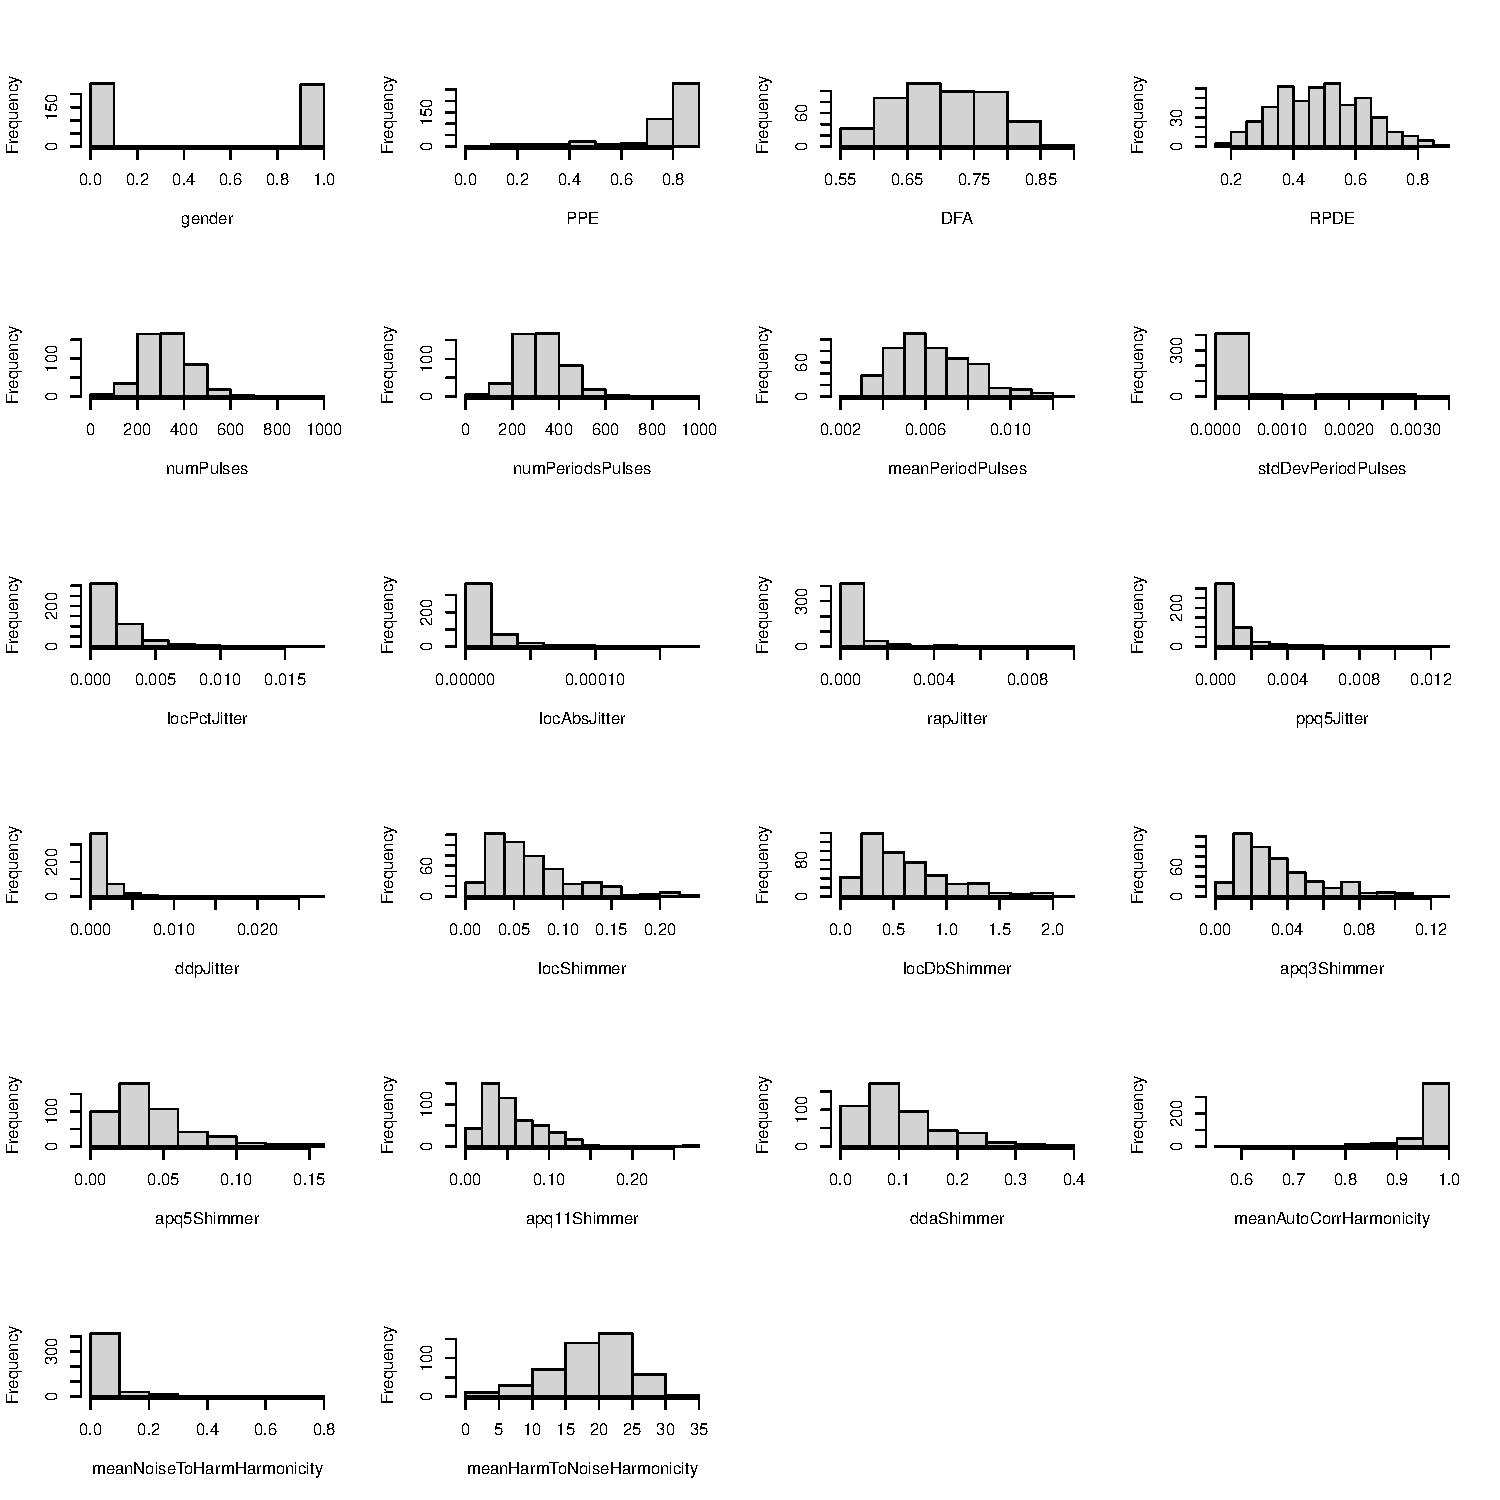
\includegraphics[width=1\linewidth,height=1\textheight]{figure/histPlots-1} 

}

\caption{\label{fig:histPlots}Pre- vs. Post-Standardization Histograms}\label{fig:histPlots-1}
\end{figure}
\begin{figure}

{\centering 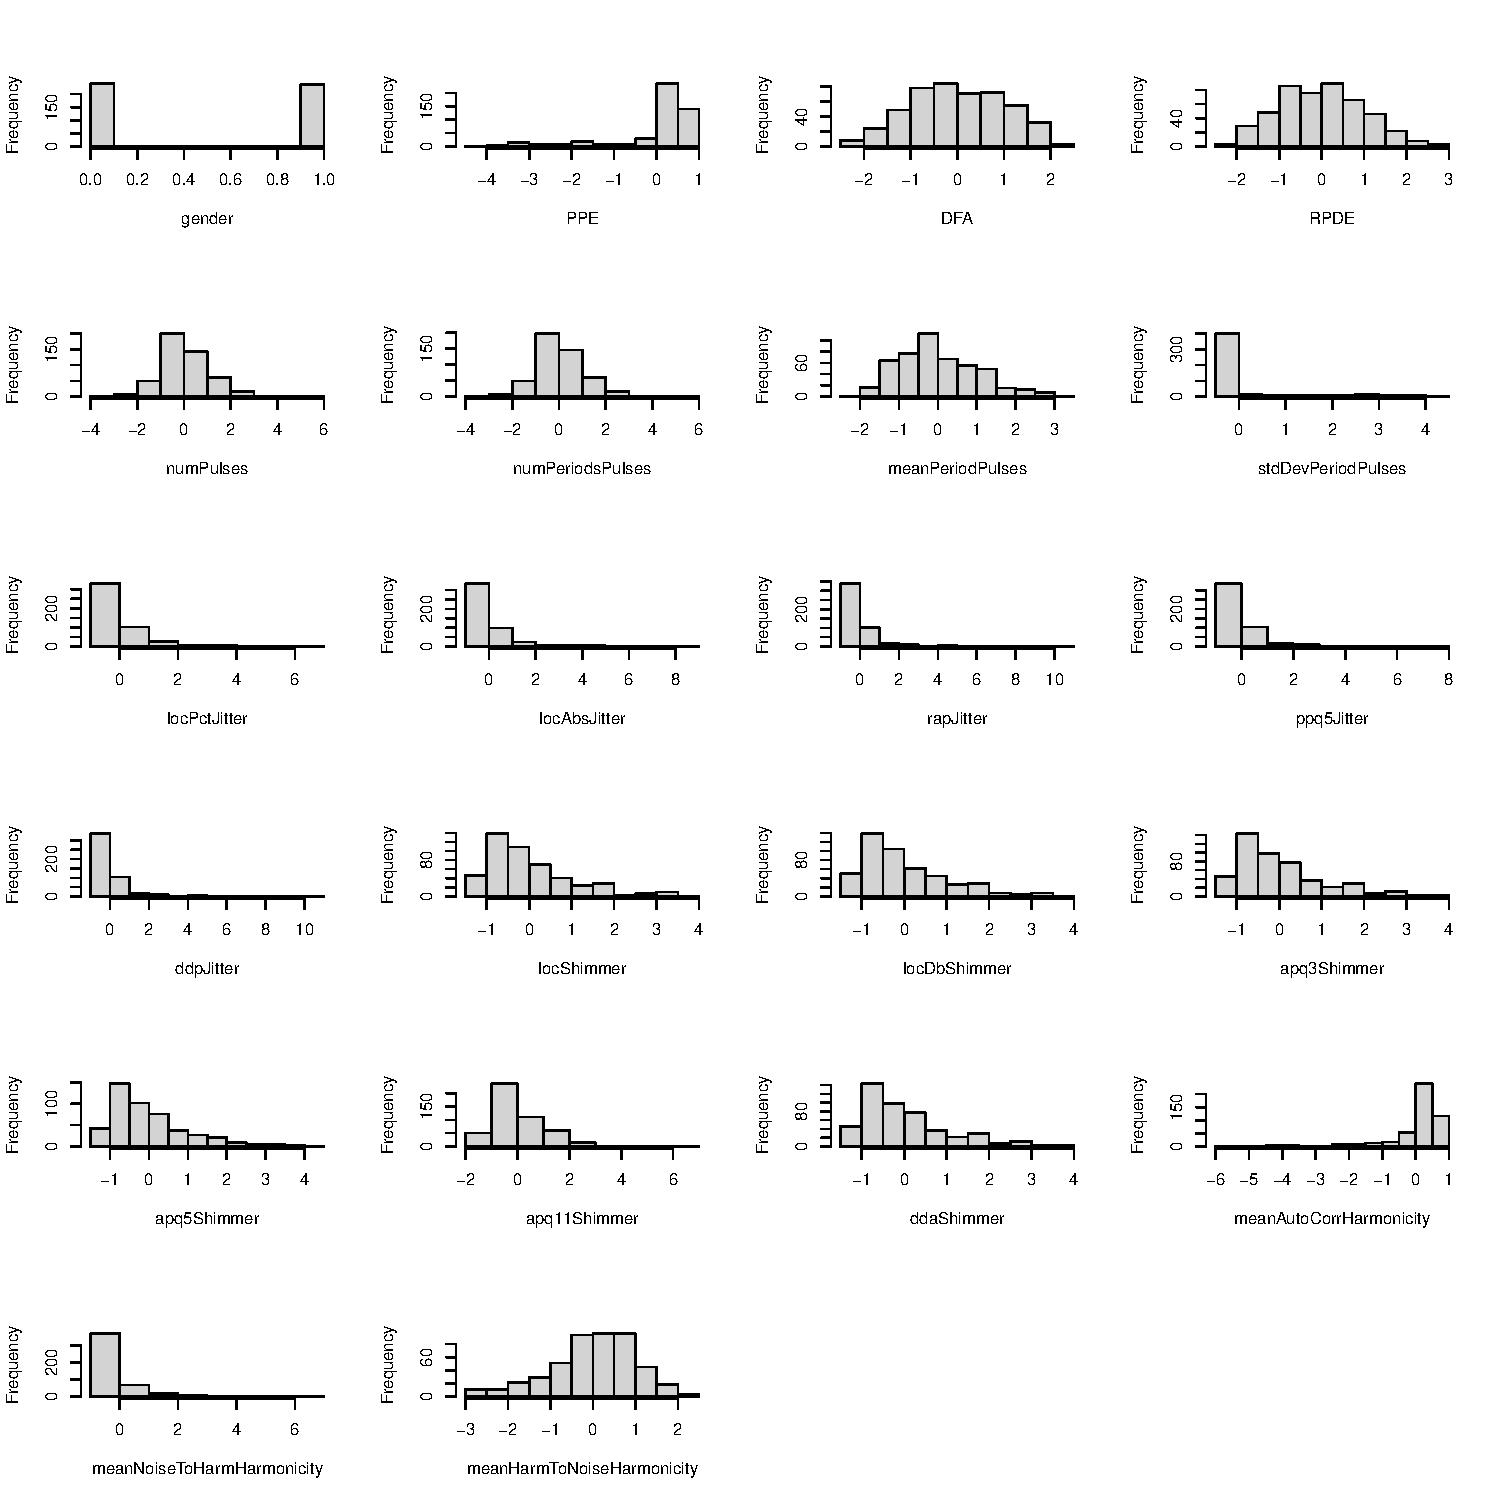
\includegraphics[width=1\linewidth,height=1\textheight]{figure/histPlots-2} 

}

\caption{\label{fig:histPlots}Pre- vs. Post-Standardization Histograms}\label{fig:histPlots-2}
\end{figure}
\begin{figure}

{\centering 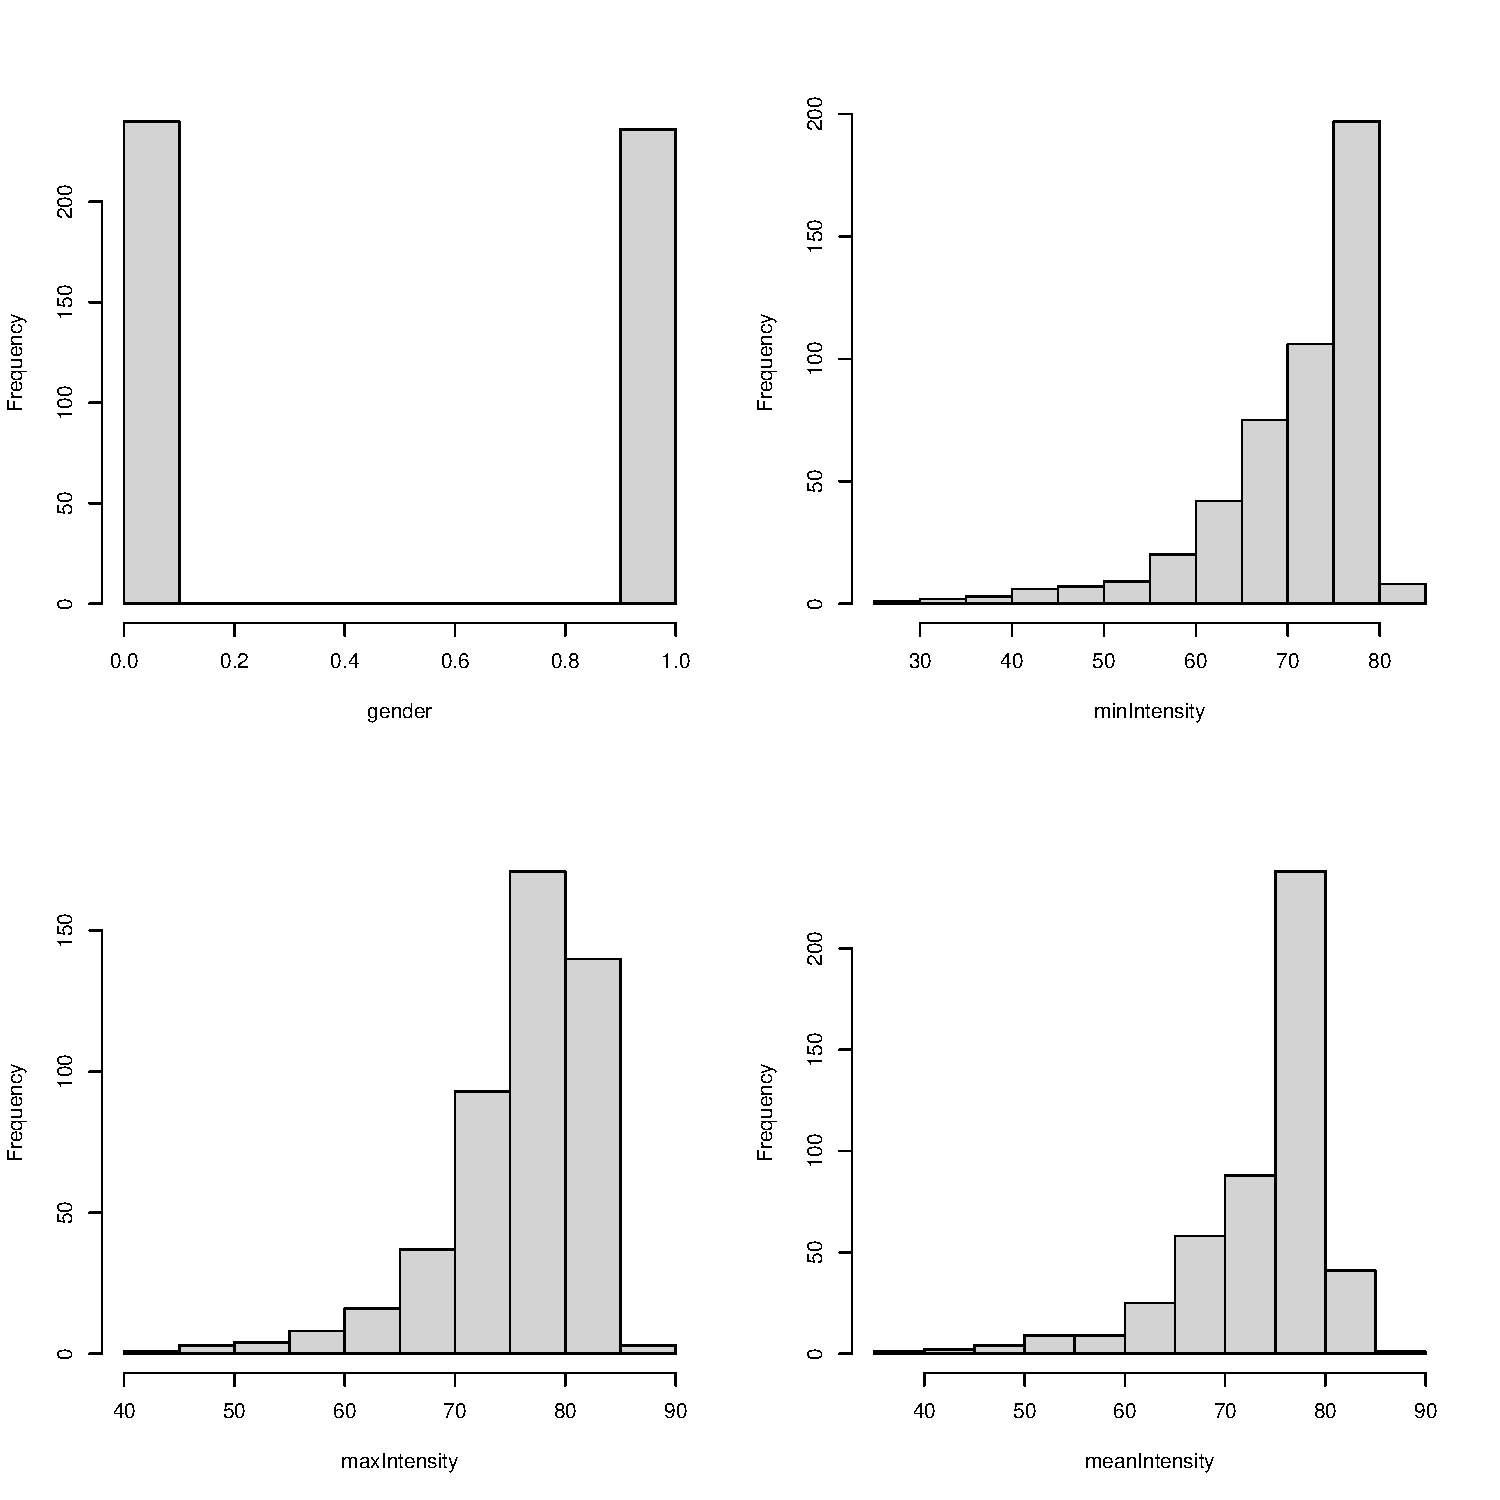
\includegraphics[width=1\linewidth,height=1\textheight]{figure/histPlots-3} 

}

\caption{\label{fig:histPlots}Pre- vs. Post-Standardization Histograms}\label{fig:histPlots-3}
\end{figure}
\begin{figure}

{\centering 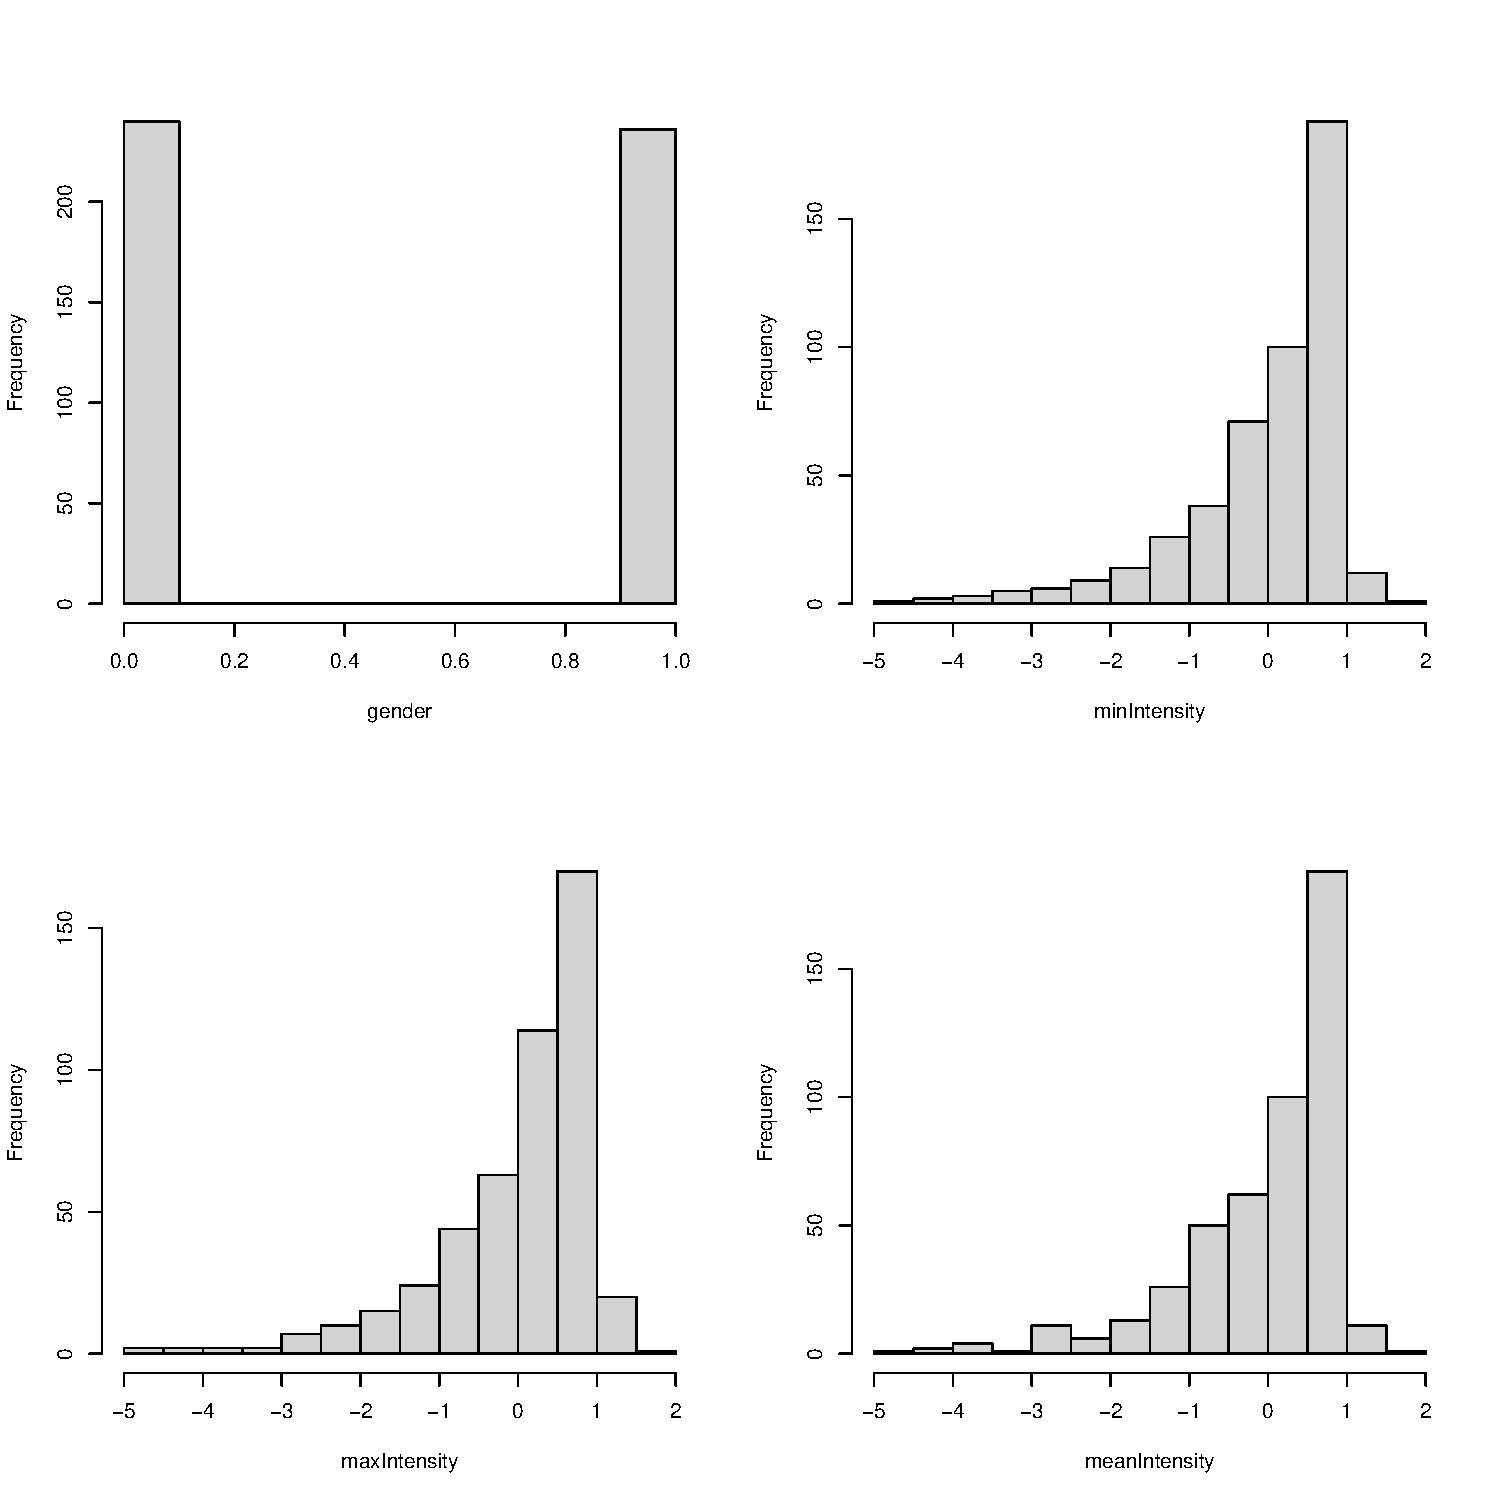
\includegraphics[width=1\linewidth,height=1\textheight]{figure/histPlots-4} 

}

\caption{\label{fig:histPlots}Pre- vs. Post-Standardization Histograms}\label{fig:histPlots-4}
\end{figure}
\begin{figure}

{\centering 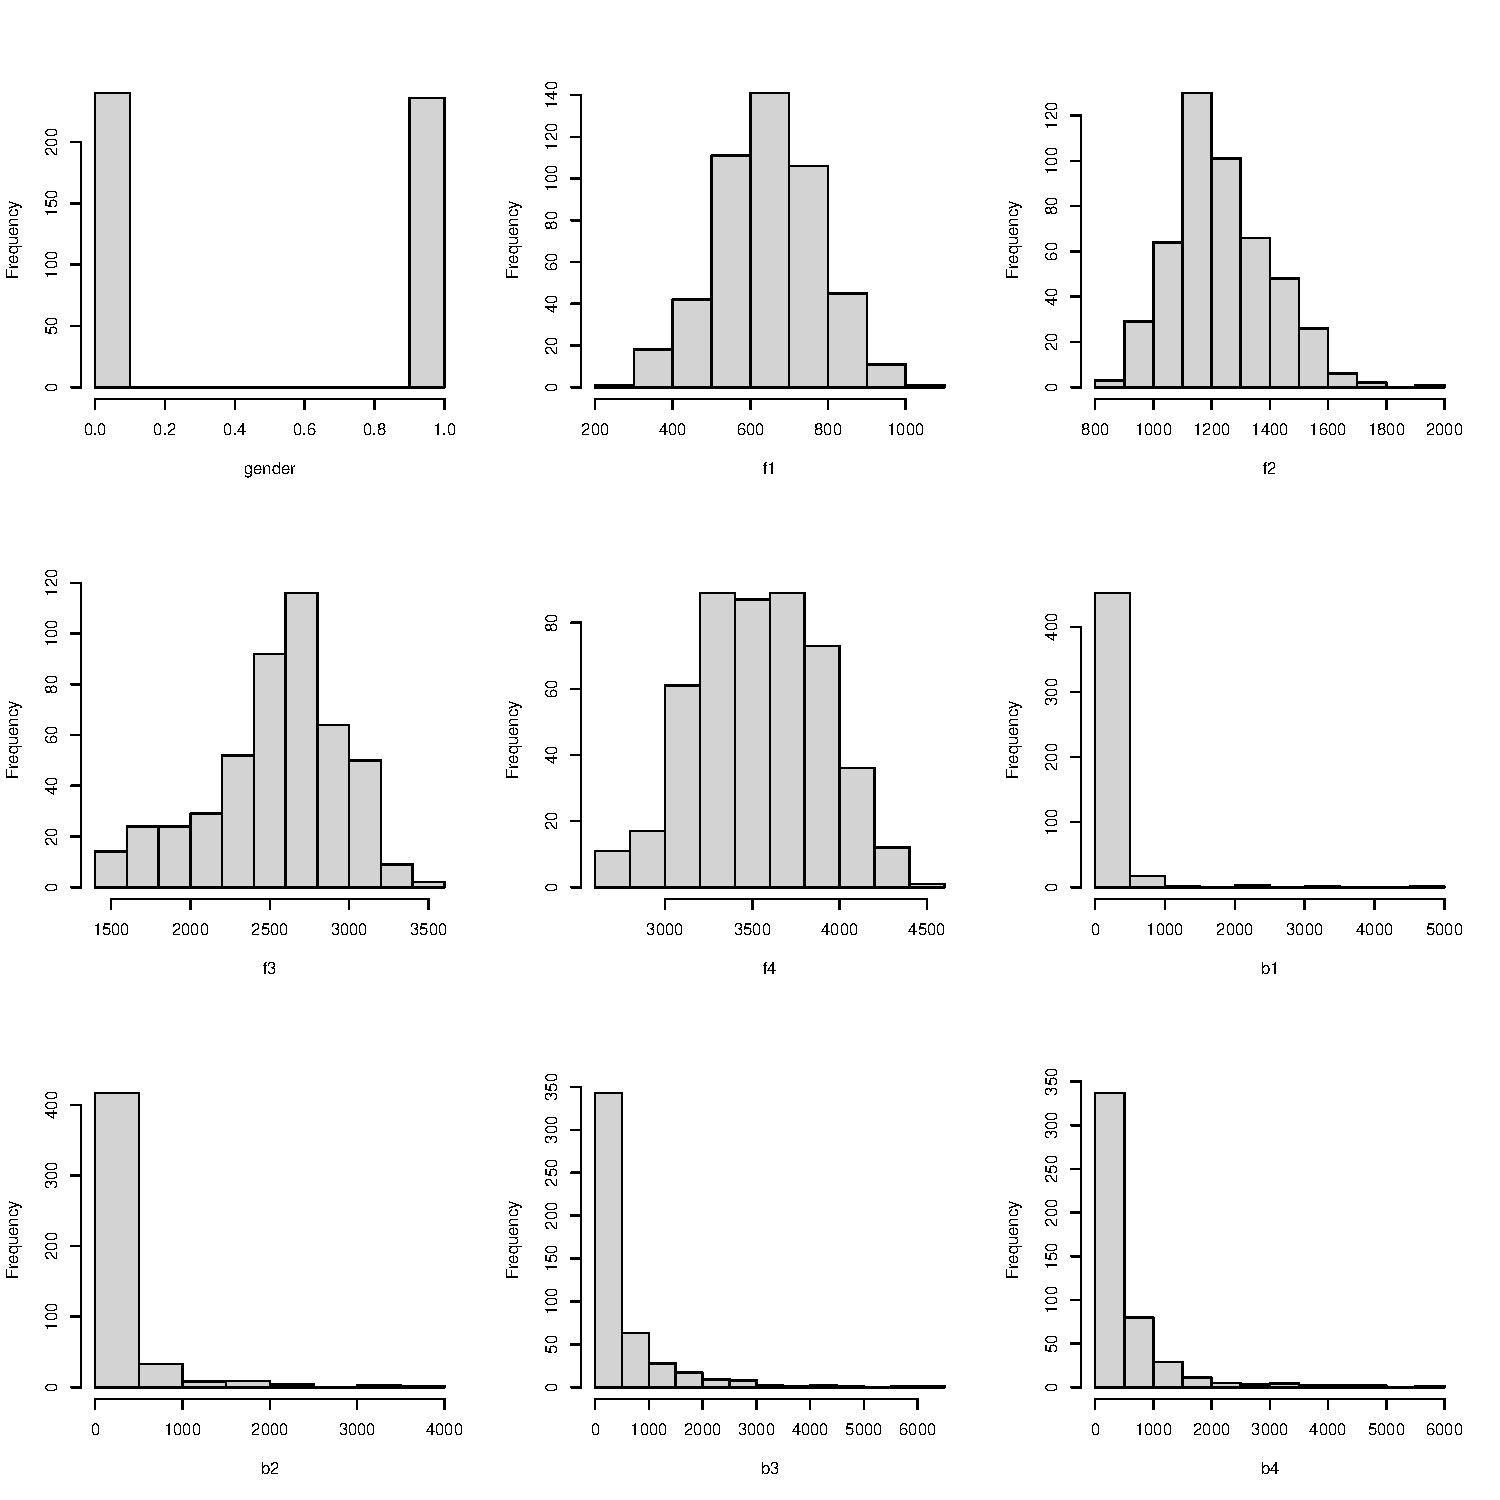
\includegraphics[width=1\linewidth,height=1\textheight]{figure/histPlots-5} 

}

\caption{\label{fig:histPlots}Pre- vs. Post-Standardization Histograms}\label{fig:histPlots-5}
\end{figure}
\begin{figure}

{\centering 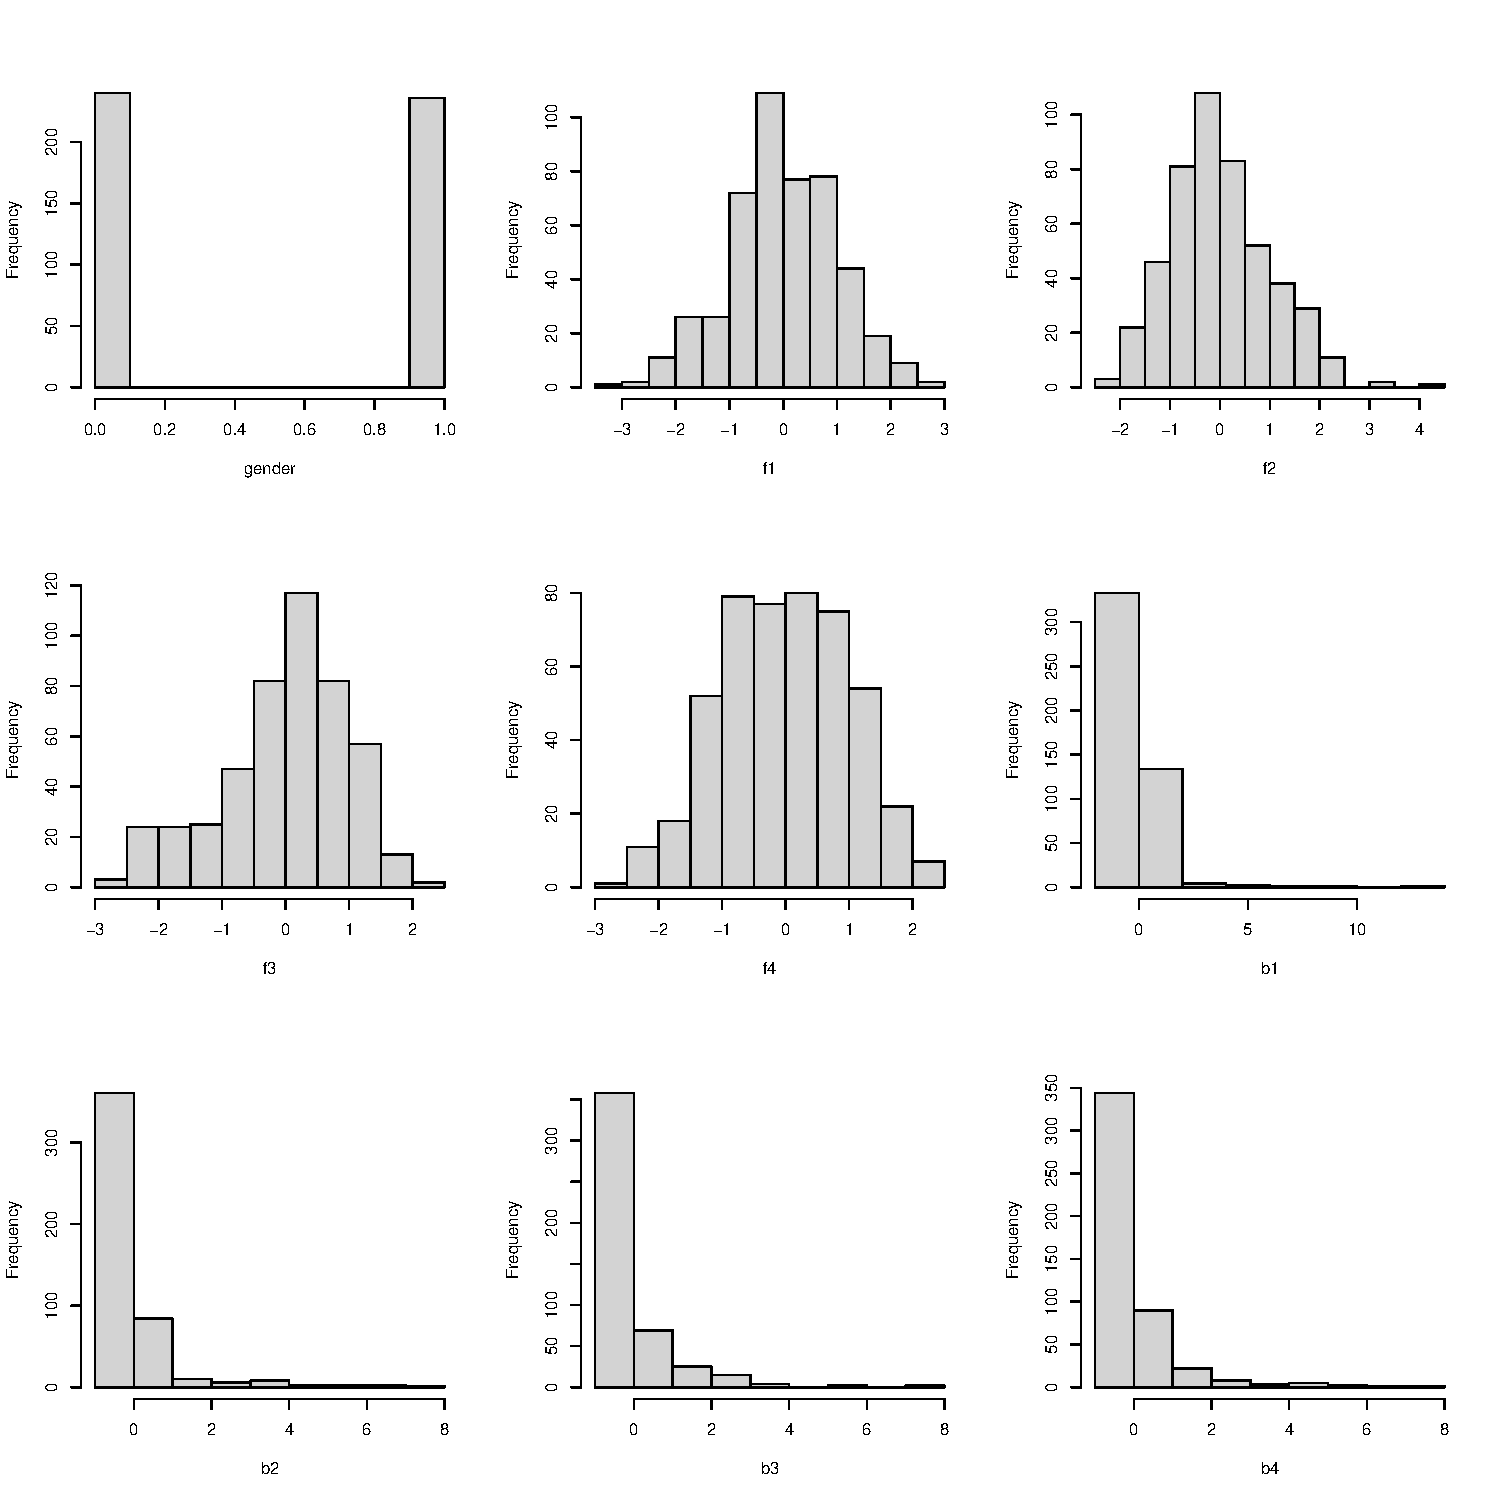
\includegraphics[width=1\linewidth,height=1\textheight]{figure/histPlots-6} 

}

\caption{\label{fig:histPlots}Pre- vs. Post-Standardization Histograms}\label{fig:histPlots-6}
\end{figure}

\newpage

\hypertarget{feature-selection}{%
\subsection{Feature Selection}\label{feature-selection}}

Per the \textbf{Sakar et al} paper, minimum redundancy-maximum relevance based filter feature selection methods are ideal for determining effective features. The advantage of this is two-fold:\\
1. It reduces the high dimensionality of the data set.
2. It maximizes the joint dependency of the data set.
This strategy is used frequenty in machine learning and regression applications, and as such, will be used in this analysis. The \textbf{Boruta} package in RStudio will be used for this purpose, and utilizes Random Forest to perform a top-down search on the corresponding data frame to determine relevant features.

\textbf{NOTE}
The Boruta algorithm takes anywhere from 7 to 30 minutes to run, depending on computing power. Please allow the model time to finish.

\begin{Shaded}
\begin{Highlighting}[]
\FunctionTok{require}\NormalTok{(Boruta)}
\FunctionTok{require}\NormalTok{(mlbench)}
\FunctionTok{require}\NormalTok{(caret)}
\FunctionTok{require}\NormalTok{(randomForest)}
\CommentTok{\# Function to perform Boruta feature selection}
\NormalTok{perform\_boruta }\OtherTok{\textless{}{-}} \ControlFlowTok{function}\NormalTok{(dataset\_name, standardized\_train\_df, }\AttributeTok{max\_runs =} \DecValTok{500}\NormalTok{) \{}
  \FunctionTok{cat}\NormalTok{(}\StringTok{"Performing Boruta on"}\NormalTok{, dataset\_name, }\StringTok{"}\SpecialCharTok{\textbackslash{}n}\StringTok{"}\NormalTok{)}
  \FunctionTok{set.seed}\NormalTok{(}\DecValTok{123}\NormalTok{)}
\NormalTok{  boruta\_result }\OtherTok{\textless{}{-}} \FunctionTok{Boruta}\NormalTok{(class }\SpecialCharTok{\textasciitilde{}}\NormalTok{ ., }\AttributeTok{data =}\NormalTok{ standardized\_train\_df, }\AttributeTok{doTrace =} \DecValTok{2}\NormalTok{, }\AttributeTok{maxRuns =}\NormalTok{ max\_runs)}
  \FunctionTok{return}\NormalTok{(boruta\_result)}
\NormalTok{\}}

\CommentTok{\# Call the perform\_boruta function for each subset. Finds important features in each subset}
\NormalTok{boruta\_results }\OtherTok{\textless{}{-}} \FunctionTok{list}\NormalTok{()}
\ControlFlowTok{for}\NormalTok{ (subset\_name }\ControlFlowTok{in}\NormalTok{ subset\_names) \{}
\NormalTok{  standardized\_train\_df }\OtherTok{\textless{}{-}} \FunctionTok{get}\NormalTok{(}\FunctionTok{paste0}\NormalTok{(}\StringTok{"train\_df\_std."}\NormalTok{, subset\_name, }\StringTok{"\_train"}\NormalTok{))}
\NormalTok{  boruta\_result }\OtherTok{\textless{}{-}} \FunctionTok{perform\_boruta}\NormalTok{(subset\_name, standardized\_train\_df)}
\NormalTok{  boruta\_results[[subset\_name]] }\OtherTok{\textless{}{-}}\NormalTok{ boruta\_result}
\NormalTok{\}}
\end{Highlighting}
\end{Shaded}

mRMR analysis yielded the following results. TQWT results are particularly dense and the plot is somewhat difficult to interpret; however, the overall trend is such that:\\
- Red regions are categorically rejected and excluded from the included features.\\
- Yellow regions are tentative, and are handled in a later section of code.\\
- Green regions are found to be important and thus selected as included features.

\begin{landscape}

\begin{figure}

{\centering 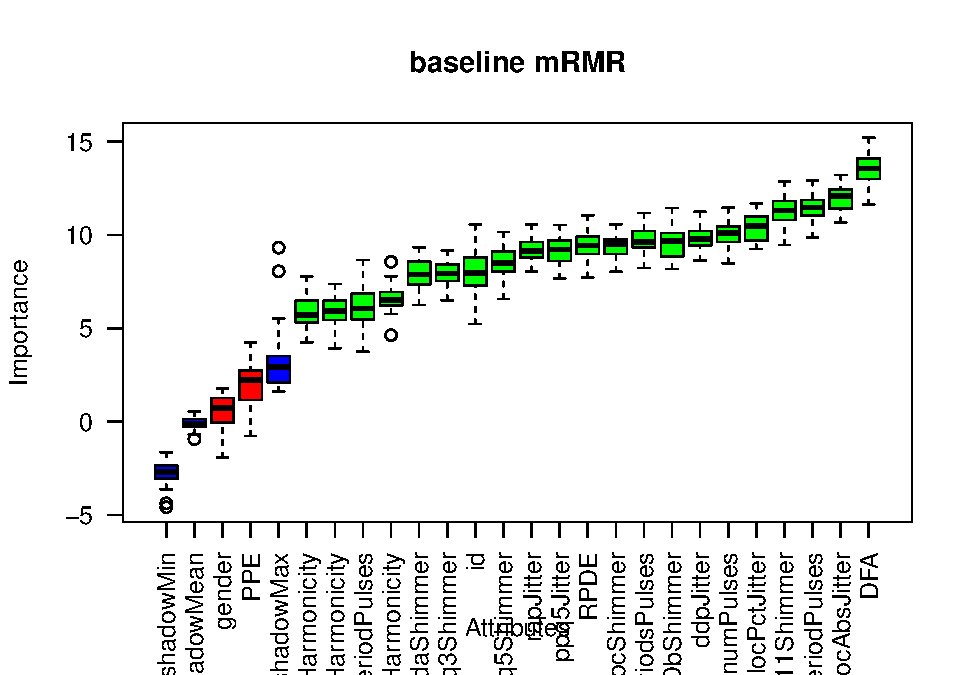
\includegraphics[width=1\linewidth,height=1\textheight]{figure/borutaPlot-1} 

}

\caption{\label{fig:borutaPlot}Boruta Plot}\label{fig:borutaPlot-1}
\end{figure}
\begin{figure}

{\centering 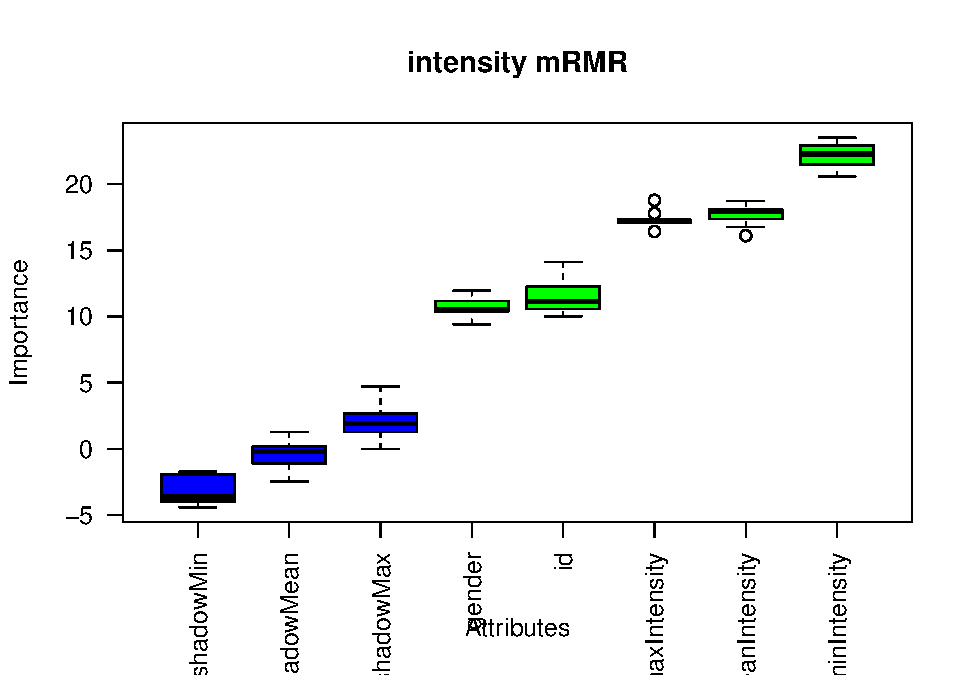
\includegraphics[width=1\linewidth,height=1\textheight]{figure/borutaPlot-2} 

}

\caption{\label{fig:borutaPlot}Boruta Plot}\label{fig:borutaPlot-2}
\end{figure}
\begin{figure}

{\centering 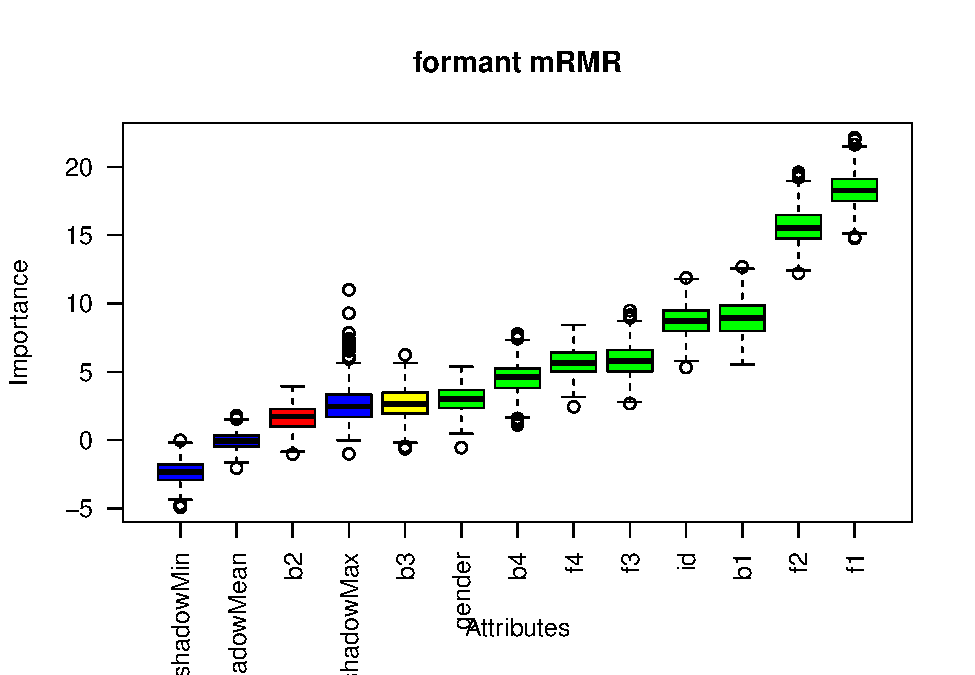
\includegraphics[width=1\linewidth,height=1\textheight]{figure/borutaPlot-3} 

}

\caption{\label{fig:borutaPlot}Boruta Plot}\label{fig:borutaPlot-3}
\end{figure}
\begin{figure}

{\centering 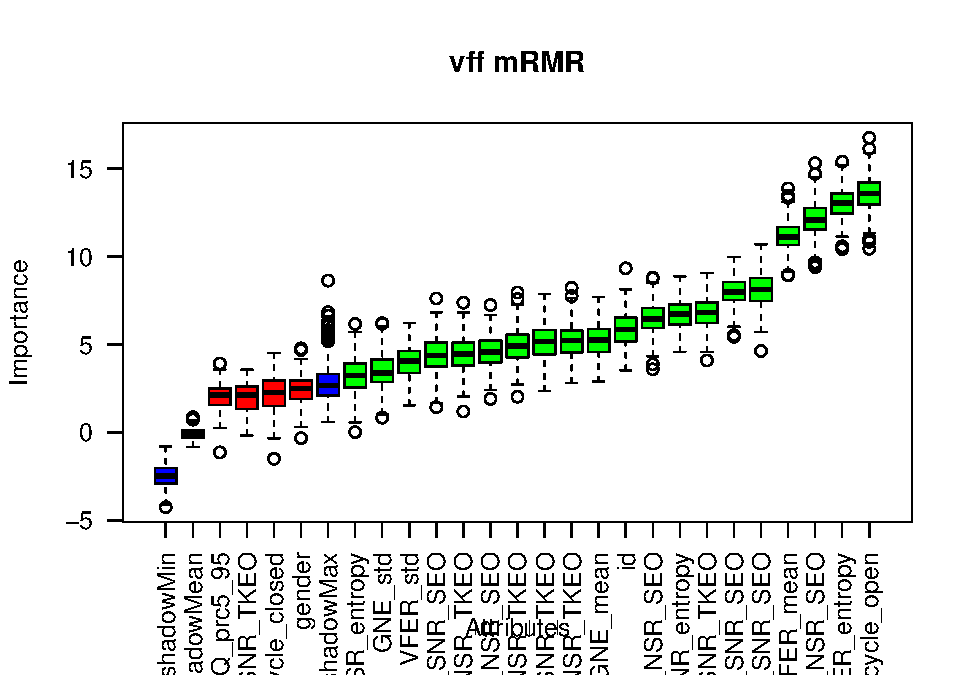
\includegraphics[width=1\linewidth,height=1\textheight]{figure/borutaPlot-4} 

}

\caption{\label{fig:borutaPlot}Boruta Plot}\label{fig:borutaPlot-4}
\end{figure}
\begin{figure}

{\centering 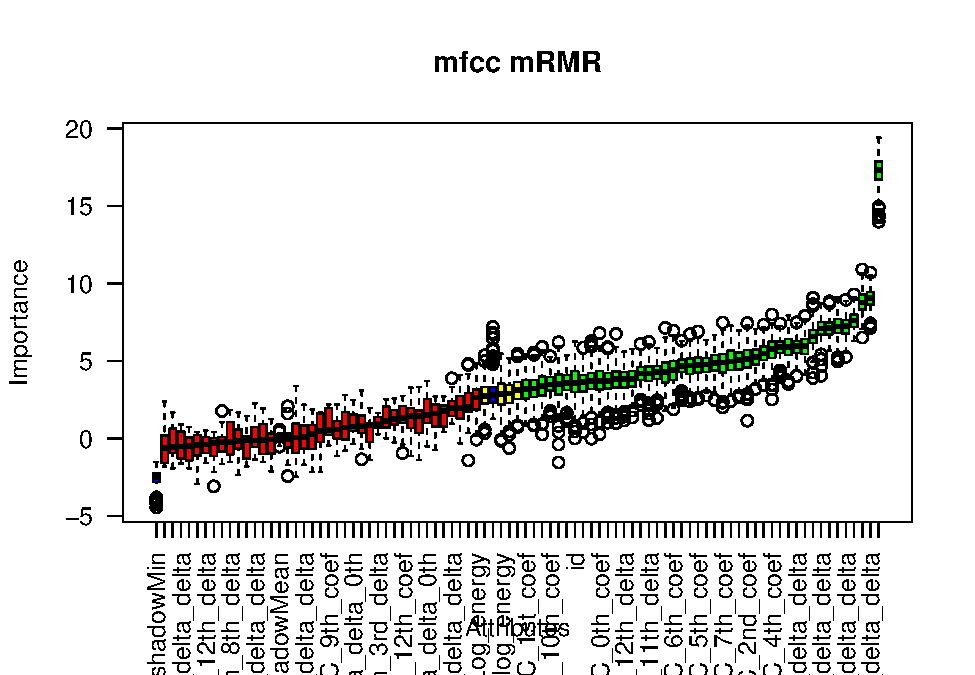
\includegraphics[width=1\linewidth,height=1\textheight]{figure/borutaPlot-5} 

}

\caption{\label{fig:borutaPlot}Boruta Plot}\label{fig:borutaPlot-5}
\end{figure}
\begin{figure}

{\centering 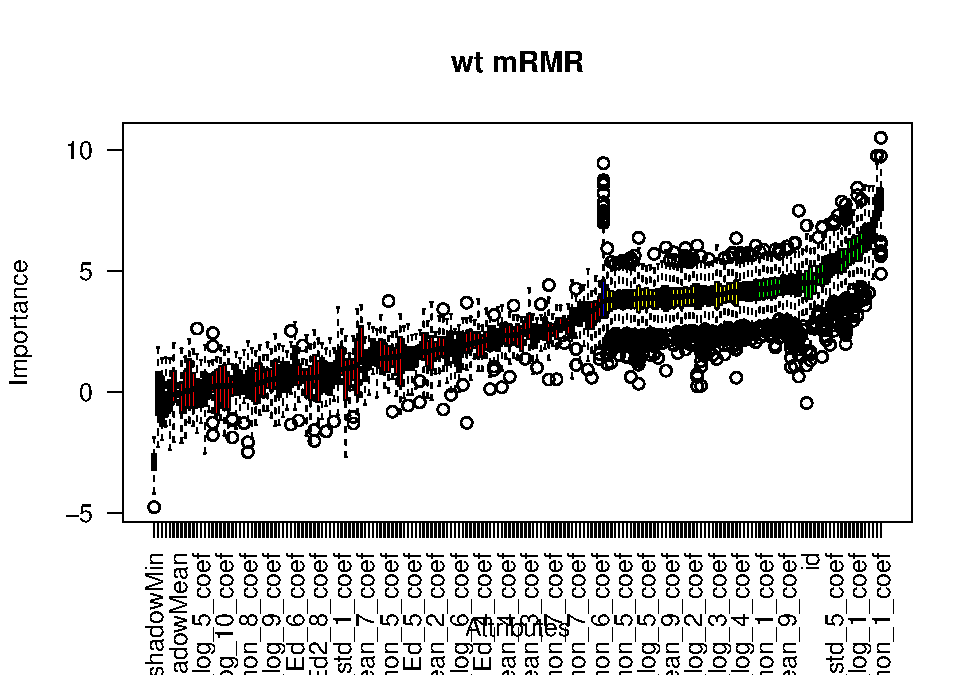
\includegraphics[width=1\linewidth,height=1\textheight]{figure/borutaPlot-6} 

}

\caption{\label{fig:borutaPlot}Boruta Plot}\label{fig:borutaPlot-6}
\end{figure}
\begin{figure}

{\centering 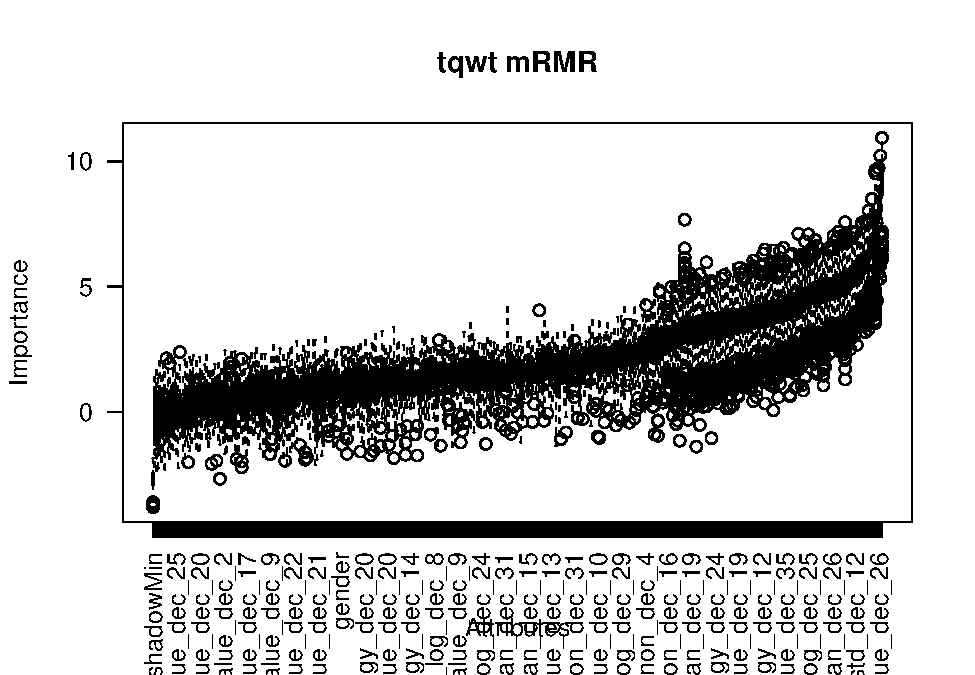
\includegraphics[width=1\linewidth,height=1\textheight]{figure/borutaPlot-7} 

}

\caption{\label{fig:borutaPlot}Boruta Plot}\label{fig:borutaPlot-7}
\end{figure}

\end{landscape}

\newpage

Following this initial assessment, chosen variables are selected for regression by using \textbf{getNonRejectedFormula()}. This collapses any variables left as \textbf{Tentative} factors into either Accepted or Rejected.

\begin{Shaded}
\begin{Highlighting}[]
\CommentTok{\#Force "Tentative" values function}
\NormalTok{get\_chosen\_features }\OtherTok{\textless{}{-}} \ControlFlowTok{function}\NormalTok{(boruta\_results) \{}
\NormalTok{  chosen\_features }\OtherTok{\textless{}{-}} \FunctionTok{list}\NormalTok{()}
  \ControlFlowTok{for}\NormalTok{ (name }\ControlFlowTok{in} \FunctionTok{names}\NormalTok{(boruta\_results)) \{}
\NormalTok{    chosen\_formula }\OtherTok{\textless{}{-}} \FunctionTok{getNonRejectedFormula}\NormalTok{(}\FunctionTok{TentativeRoughFix}\NormalTok{(boruta\_results[[name]]))}
\NormalTok{    chosen\_features[[name]] }\OtherTok{\textless{}{-}}\NormalTok{ chosen\_formula}
\NormalTok{  \}}
  \FunctionTok{return}\NormalTok{(chosen\_features)}
\NormalTok{\}}
\end{Highlighting}
\end{Shaded}

The following factors were found to be important to the model:

\begin{table}
\centering\begingroup\fontsize{5}{7}\selectfont

\begin{tabular}{cccc}
\toprule
Column 1 & Column 2 & Column 3 & Column 4\\
\midrule
class & id & DFA & RPDE\\
numPulses & numPeriodsPulses & meanPeriodPulses & stdDevPeriodPulses\\
locPctJitter & locAbsJitter & rapJitter & ppq5Jitter\\
ddpJitter & locShimmer & locDbShimmer & apq3Shimmer\\
apq5Shimmer & apq11Shimmer & ddaShimmer & meanAutoCorrHarmonicity\\
\addlinespace
meanNoiseToHarmHarmonicity & meanHarmToNoiseHarmonicity & gender & minIntensity\\
maxIntensity & meanIntensity & f1 & f2\\
f3 & f4 & b1 & b3\\
b4 & GQ\_std\_cycle\_open & GNE\_mean & GNE\_std\\
GNE\_SNR\_TKEO & GNE\_SNR\_SEO & GNE\_NSR\_TKEO & GNE\_NSR\_SEO\\
\addlinespace
VFER\_mean & VFER\_std & VFER\_entropy & VFER\_SNR\_TKEO\\
VFER\_SNR\_SEO & VFER\_NSR\_TKEO & VFER\_NSR\_SEO & IMF\_SNR\_SEO\\
IMF\_SNR\_entropy & IMF\_NSR\_SEO & IMF\_NSR\_TKEO & IMF\_NSR\_entropy\\
mean\_MFCC\_0th\_coef & mean\_MFCC\_1st\_coef & mean\_MFCC\_2nd\_coef & mean\_MFCC\_3rd\_coef\\
mean\_MFCC\_4th\_coef & mean\_MFCC\_5th\_coef & mean\_MFCC\_6th\_coef & mean\_MFCC\_7th\_coef\\
\addlinespace
mean\_delta\_log\_energy & mean\_2nd\_delta & std\_Log\_energy & std\_MFCC\_1st\_coef\\
std\_MFCC\_2nd\_coef & std\_MFCC\_3rd\_coef & std\_MFCC\_4th\_coef & std\_MFCC\_5th\_coef\\
std\_MFCC\_6th\_coef & std\_MFCC\_7th\_coef & std\_MFCC\_8th\_coef & std\_MFCC\_10th\_coef\\
std\_MFCC\_11th\_coef & std\_delta\_log\_energy & std\_1st\_delta & std\_2nd\_delta\\
std\_3rd\_delta & std\_4th\_delta & std\_5th\_delta & std\_6th\_delta\\
\addlinespace
std\_7th\_delta & std\_8th\_delta & std\_9th\_delta & std\_10th\_delta\\
std\_11th\_delta & std\_12th\_delta & std\_delta\_delta\_log\_energy & std\_1st\_delta\_delta\\
std\_3rd\_delta\_delta & std\_4th\_delta\_delta & std\_5th\_delta\_delta & std\_6th\_delta\_delta\\
std\_7th\_delta\_delta & std\_8th\_delta\_delta & std\_9th\_delta\_delta & std\_10th\_delta\_delta\\
std\_11th\_delta\_delta & std\_12th\_delta\_delta & Ed\_1\_coef & Ed\_2\_coef\\
\addlinespace
Ed\_3\_coef & det\_entropy\_shannon\_3\_coef & det\_entropy\_log\_1\_coef & det\_entropy\_log\_2\_coef\\
det\_entropy\_log\_3\_coef & det\_TKEO\_mean\_1\_coef & det\_TKEO\_std\_1\_coef & det\_TKEO\_std\_3\_coef\\
app\_entropy\_shannon\_1\_coef & app\_entropy\_shannon\_2\_coef & app\_entropy\_shannon\_3\_coef & app\_entropy\_shannon\_4\_coef\\
app\_entropy\_shannon\_5\_coef & app\_entropy\_shannon\_9\_coef & app\_entropy\_log\_1\_coef & app\_entropy\_log\_2\_coef\\
app\_entropy\_log\_3\_coef & app\_entropy\_log\_4\_coef & app\_entropy\_log\_5\_coef & app\_entropy\_log\_6\_coef\\
\addlinespace
app\_entropy\_log\_9\_coef & app\_entropy\_log\_10\_coef & app\_det\_TKEO\_mean\_4\_coef & app\_det\_TKEO\_mean\_5\_coef\\
app\_det\_TKEO\_mean\_8\_coef & app\_det\_TKEO\_mean\_9\_coef & app\_det\_TKEO\_mean\_10\_coef & app\_TKEO\_std\_5\_coef\\
app\_TKEO\_std\_6\_coef & app\_TKEO\_std\_10\_coef & Ed2\_1\_coef & Ed2\_2\_coef\\
Ed2\_3\_coef & det\_LT\_entropy\_shannon\_1\_coef & det\_LT\_entropy\_shannon\_3\_coef & det\_LT\_entropy\_log\_1\_coef\\
det\_LT\_entropy\_log\_3\_coef & det\_LT\_TKEO\_mean\_1\_coef & det\_LT\_TKEO\_mean\_3\_coef & det\_LT\_TKEO\_std\_1\_coef\\
\addlinespace
det\_LT\_TKEO\_std\_2\_coef & det\_LT\_TKEO\_std\_3\_coef & app\_LT\_entropy\_shannon\_1\_coef & app\_LT\_entropy\_shannon\_2\_coef\\
app\_LT\_entropy\_shannon\_3\_coef & app\_LT\_entropy\_shannon\_4\_coef & app\_LT\_entropy\_shannon\_5\_coef & app\_LT\_entropy\_shannon\_6\_coef\\
app\_LT\_entropy\_shannon\_8\_coef & app\_LT\_entropy\_shannon\_10\_coef & app\_LT\_entropy\_log\_1\_coef & app\_LT\_entropy\_log\_2\_coef\\
app\_LT\_entropy\_log\_3\_coef & app\_LT\_entropy\_log\_4\_coef & app\_LT\_entropy\_log\_5\_coef & app\_LT\_entropy\_log\_6\_coef\\
app\_LT\_entropy\_log\_8\_coef & app\_LT\_entropy\_log\_9\_coef & app\_LT\_entropy\_log\_10\_coef & app\_LT\_TKEO\_mean\_8\_coef\\
\addlinespace
app\_LT\_TKEO\_mean\_9\_coef & app\_LT\_TKEO\_mean\_10\_coef & app\_LT\_TKEO\_std\_5\_coef & app\_LT\_TKEO\_std\_6\_coef\\
app\_LT\_TKEO\_std\_7\_coef & app\_LT\_TKEO\_std\_8\_coef & app\_LT\_TKEO\_std\_9\_coef & app\_LT\_TKEO\_std\_10\_coef\\
tqwt\_energy\_dec\_1 & tqwt\_energy\_dec\_2 & tqwt\_energy\_dec\_6 & tqwt\_energy\_dec\_11\\
tqwt\_energy\_dec\_12 & tqwt\_energy\_dec\_18 & tqwt\_energy\_dec\_24 & tqwt\_energy\_dec\_25\\
tqwt\_energy\_dec\_26 & tqwt\_energy\_dec\_27 & tqwt\_energy\_dec\_28 & tqwt\_energy\_dec\_33\\
\addlinespace
tqwt\_energy\_dec\_34 & tqwt\_energy\_dec\_35 & tqwt\_entropy\_shannon\_dec\_1 & tqwt\_entropy\_shannon\_dec\_6\\
tqwt\_entropy\_shannon\_dec\_11 & tqwt\_entropy\_shannon\_dec\_12 & tqwt\_entropy\_shannon\_dec\_13 & tqwt\_entropy\_shannon\_dec\_14\\
tqwt\_entropy\_shannon\_dec\_15 & tqwt\_entropy\_shannon\_dec\_32 & tqwt\_entropy\_shannon\_dec\_33 & tqwt\_entropy\_shannon\_dec\_34\\
tqwt\_entropy\_shannon\_dec\_35 & tqwt\_entropy\_shannon\_dec\_36 & tqwt\_entropy\_log\_dec\_1 & tqwt\_entropy\_log\_dec\_12\\
tqwt\_entropy\_log\_dec\_13 & tqwt\_entropy\_log\_dec\_16 & tqwt\_entropy\_log\_dec\_18 & tqwt\_entropy\_log\_dec\_19\\
\addlinespace
tqwt\_entropy\_log\_dec\_25 & tqwt\_entropy\_log\_dec\_26 & tqwt\_entropy\_log\_dec\_27 & tqwt\_entropy\_log\_dec\_28\\
tqwt\_entropy\_log\_dec\_32 & tqwt\_entropy\_log\_dec\_33 & tqwt\_entropy\_log\_dec\_34 & tqwt\_entropy\_log\_dec\_35\\
tqwt\_TKEO\_mean\_dec\_2 & tqwt\_TKEO\_mean\_dec\_6 & tqwt\_TKEO\_mean\_dec\_11 & tqwt\_TKEO\_mean\_dec\_12\\
tqwt\_TKEO\_mean\_dec\_13 & tqwt\_TKEO\_mean\_dec\_18 & tqwt\_TKEO\_mean\_dec\_19 & tqwt\_TKEO\_mean\_dec\_25\\
tqwt\_TKEO\_mean\_dec\_26 & tqwt\_TKEO\_mean\_dec\_27 & tqwt\_TKEO\_mean\_dec\_32 & tqwt\_TKEO\_mean\_dec\_33\\
\addlinespace
tqwt\_TKEO\_mean\_dec\_34 & tqwt\_TKEO\_mean\_dec\_35 & tqwt\_TKEO\_std\_dec\_6 & tqwt\_TKEO\_std\_dec\_8\\
tqwt\_TKEO\_std\_dec\_11 & tqwt\_TKEO\_std\_dec\_12 & tqwt\_TKEO\_std\_dec\_13 & tqwt\_TKEO\_std\_dec\_14\\
tqwt\_TKEO\_std\_dec\_17 & tqwt\_TKEO\_std\_dec\_19 & tqwt\_TKEO\_std\_dec\_25 & tqwt\_TKEO\_std\_dec\_26\\
tqwt\_TKEO\_std\_dec\_34 & tqwt\_medianValue\_dec\_31 & tqwt\_medianValue\_dec\_34 & tqwt\_meanValue\_dec\_34\\
tqwt\_meanValue\_dec\_36 & tqwt\_stdValue\_dec\_1 & tqwt\_stdValue\_dec\_2 & tqwt\_stdValue\_dec\_5\\
\addlinespace
tqwt\_stdValue\_dec\_6 & tqwt\_stdValue\_dec\_7 & tqwt\_stdValue\_dec\_11 & tqwt\_stdValue\_dec\_12\\
tqwt\_stdValue\_dec\_13 & tqwt\_stdValue\_dec\_18 & tqwt\_stdValue\_dec\_19 & tqwt\_stdValue\_dec\_25\\
tqwt\_stdValue\_dec\_26 & tqwt\_stdValue\_dec\_27 & tqwt\_stdValue\_dec\_32 & tqwt\_stdValue\_dec\_33\\
tqwt\_stdValue\_dec\_34 & tqwt\_stdValue\_dec\_35 & tqwt\_minValue\_dec\_7 & tqwt\_minValue\_dec\_11\\
tqwt\_minValue\_dec\_12 & tqwt\_minValue\_dec\_13 & tqwt\_minValue\_dec\_14 & tqwt\_minValue\_dec\_17\\
\addlinespace
tqwt\_maxValue\_dec\_6 & tqwt\_maxValue\_dec\_11 & tqwt\_maxValue\_dec\_12 & tqwt\_maxValue\_dec\_13\\
tqwt\_maxValue\_dec\_14 & tqwt\_maxValue\_dec\_17 & tqwt\_skewnessValue\_dec\_24 & tqwt\_skewnessValue\_dec\_25\\
tqwt\_skewnessValue\_dec\_26 & tqwt\_skewnessValue\_dec\_27 & tqwt\_kurtosisValue\_dec\_12 & tqwt\_kurtosisValue\_dec\_16\\
tqwt\_kurtosisValue\_dec\_17 & tqwt\_kurtosisValue\_dec\_18 & tqwt\_kurtosisValue\_dec\_19 & tqwt\_kurtosisValue\_dec\_20\\
tqwt\_kurtosisValue\_dec\_22 & tqwt\_kurtosisValue\_dec\_25 & tqwt\_kurtosisValue\_dec\_26 & tqwt\_kurtosisValue\_dec\_27\\
\addlinespace
tqwt\_kurtosisValue\_dec\_29 & tqwt\_kurtosisValue\_dec\_32 & tqwt\_kurtosisValue\_dec\_33 & tqwt\_kurtosisValue\_dec\_34\\
tqwt\_kurtosisValue\_dec\_35 & NA & NA & NA\\
\bottomrule
\end{tabular}
\endgroup{}
\end{table}
\newpage

\hypertarget{model-selection-and-weighting}{%
\subsection{Model Selection and Weighting}\label{model-selection-and-weighting}}

Once the important features had been determined, they can be used to inform the predictive model for each sub-group.
For this analysis, a function was built to test each sub-group against a number of predictive models. Using the 10\% ``test'' data of the training set, accuracy estimates were generated and used to benchmark the model's performance against each other. The models used for analysis were:

\begin{itemize}
\tightlist
\item
  Multilayer Perceptron\\
\item
  Logistic Regression\\
\item
  Random Forest\\
\item
  SVM w/ Linear Kernel\\
\item
  SVM w/ Radial Kernel
\item
  Naive Bayes\\
\item
  k- Nearest Neighbors
\end{itemize}

\begin{Shaded}
\begin{Highlighting}[]
\CommentTok{\#Function for Multilayer Perceptron}
\NormalTok{train\_mlp }\OtherTok{\textless{}{-}} \ControlFlowTok{function}\NormalTok{(train\_df, formula) \{}
  \FunctionTok{library}\NormalTok{(neuralnet)}
  \FunctionTok{set.seed}\NormalTok{(}\DecValTok{123}\NormalTok{)}
  
\NormalTok{  threshold\_func }\OtherTok{\textless{}{-}} \ControlFlowTok{function}\NormalTok{(x) }\FunctionTok{ifelse}\NormalTok{(x }\SpecialCharTok{\textgreater{}} \FloatTok{0.5}\NormalTok{, }\DecValTok{1}\NormalTok{, }\DecValTok{0}\NormalTok{)}
\NormalTok{  train\_df}\SpecialCharTok{$}\NormalTok{class }\OtherTok{\textless{}{-}} \FunctionTok{as.numeric}\NormalTok{(train\_df}\SpecialCharTok{$}\NormalTok{class) }\SpecialCharTok{{-}} \DecValTok{1}
  
\NormalTok{  mlp\_model }\OtherTok{\textless{}{-}} \FunctionTok{neuralnet}\NormalTok{(formula, }\AttributeTok{data =}\NormalTok{ train\_df, }\AttributeTok{hidden =} \FunctionTok{c}\NormalTok{(}\DecValTok{5}\NormalTok{), }\AttributeTok{linear.output =} \ConstantTok{FALSE}\NormalTok{, }\AttributeTok{act.fct =} \StringTok{"logistic"}\NormalTok{, }\AttributeTok{stepmax =} \FloatTok{1e+05}\NormalTok{)}
  \FunctionTok{return}\NormalTok{(}\FunctionTok{list}\NormalTok{(}\AttributeTok{model =}\NormalTok{ mlp\_model, }\AttributeTok{threshold\_func =}\NormalTok{ threshold\_func))}
\NormalTok{\}}

\NormalTok{test\_model }\OtherTok{\textless{}{-}} \ControlFlowTok{function}\NormalTok{(model\_obj, test\_df, model\_type, chosen\_formula) \{}
  \ControlFlowTok{if}\NormalTok{ (model\_type }\SpecialCharTok{==} \StringTok{"mlp"}\NormalTok{) \{}
\NormalTok{    model }\OtherTok{\textless{}{-}}\NormalTok{ model\_obj}\SpecialCharTok{$}\NormalTok{model}
\NormalTok{    threshold\_func }\OtherTok{\textless{}{-}}\NormalTok{ model\_obj}\SpecialCharTok{$}\NormalTok{threshold\_func}
    
\NormalTok{    test\_data }\OtherTok{\textless{}{-}} \FunctionTok{model.matrix}\NormalTok{(chosen\_formula, }\AttributeTok{data =}\NormalTok{ test\_df)[, }\SpecialCharTok{{-}}\DecValTok{1}\NormalTok{]}
\NormalTok{    predictions }\OtherTok{\textless{}{-}} \FunctionTok{compute}\NormalTok{(model, test\_data)}\SpecialCharTok{$}\NormalTok{net.result}
\NormalTok{    predicted\_classes }\OtherTok{\textless{}{-}} \FunctionTok{sapply}\NormalTok{(predictions, threshold\_func)}
\NormalTok{    actual\_classes }\OtherTok{\textless{}{-}}\NormalTok{ test\_df}\SpecialCharTok{$}\NormalTok{class}
    
\NormalTok{    accuracy }\OtherTok{\textless{}{-}} \FunctionTok{sum}\NormalTok{(predicted\_classes }\SpecialCharTok{==}\NormalTok{ actual\_classes) }\SpecialCharTok{/} \FunctionTok{length}\NormalTok{(actual\_classes)}
\NormalTok{  \} }\ControlFlowTok{else}\NormalTok{ \{}
\NormalTok{    predictions }\OtherTok{\textless{}{-}} \FunctionTok{predict}\NormalTok{(model\_obj, test\_df)}
    
    \ControlFlowTok{if}\NormalTok{ (model\_type }\SpecialCharTok{\%in\%} \FunctionTok{c}\NormalTok{(}\StringTok{"logit"}\NormalTok{, }\StringTok{"svm\_linear"}\NormalTok{, }\StringTok{"svm\_rbf"}\NormalTok{)) \{}
\NormalTok{      predicted\_classes }\OtherTok{\textless{}{-}} \FunctionTok{ifelse}\NormalTok{(predictions }\SpecialCharTok{\textgreater{}} \FloatTok{0.5}\NormalTok{, }\DecValTok{1}\NormalTok{, }\DecValTok{0}\NormalTok{)}
\NormalTok{    \} }\ControlFlowTok{else}\NormalTok{ \{}
\NormalTok{      predicted\_classes }\OtherTok{\textless{}{-}}\NormalTok{ predictions}
\NormalTok{    \}}
\NormalTok{    actual\_classes }\OtherTok{\textless{}{-}}\NormalTok{ test\_df}\SpecialCharTok{$}\NormalTok{class}
    
\NormalTok{    accuracy }\OtherTok{\textless{}{-}} \FunctionTok{sum}\NormalTok{(predicted\_classes }\SpecialCharTok{==}\NormalTok{ actual\_classes) }\SpecialCharTok{/} \FunctionTok{length}\NormalTok{(actual\_classes)}
\NormalTok{  \}}
  
  \FunctionTok{return}\NormalTok{(accuracy)}
\NormalTok{\}}
\end{Highlighting}
\end{Shaded}

For this analysis it required the use of the \textbf{caret}, \textbf{randomForest}, \textbf{e1071}, \textbf{nnet}, \textbf{kernlab}, and \textbf{naivebayes} libraries.

\begin{Shaded}
\begin{Highlighting}[]
\CommentTok{\#Modeling function}
\NormalTok{generate\_models }\OtherTok{\textless{}{-}} \ControlFlowTok{function}\NormalTok{(dataset\_name, train\_df, test\_df) \{}
  \FunctionTok{library}\NormalTok{(caret)}
  \FunctionTok{library}\NormalTok{(randomForest)}
  \FunctionTok{library}\NormalTok{(e1071)}
  \FunctionTok{library}\NormalTok{(nnet)}
  \FunctionTok{library}\NormalTok{(kernlab)}
  \FunctionTok{library}\NormalTok{(naivebayes)}
  
  \FunctionTok{set.seed}\NormalTok{(}\DecValTok{123}\NormalTok{)}
  \CommentTok{\# Create chosen\_formula}
\NormalTok{  chosen\_formula }\OtherTok{\textless{}{-}} \FunctionTok{as.formula}\NormalTok{(chosen\_features[[dataset\_name]])}

  \CommentTok{\# Convert the class variable into a factor}
\NormalTok{  train\_df}\SpecialCharTok{$}\NormalTok{class }\OtherTok{\textless{}{-}} \FunctionTok{as.factor}\NormalTok{(train\_df}\SpecialCharTok{$}\NormalTok{class)}
\NormalTok{  test\_df}\SpecialCharTok{$}\NormalTok{class }\OtherTok{\textless{}{-}} \FunctionTok{as.factor}\NormalTok{(test\_df}\SpecialCharTok{$}\NormalTok{class)}

  \CommentTok{\# Create chosen\_formula}
\NormalTok{  chosen\_formula }\OtherTok{\textless{}{-}} \FunctionTok{as.formula}\NormalTok{(chosen\_features[[dataset\_name]])}

  \CommentTok{\# Train/test data}
\NormalTok{  train\_data }\OtherTok{\textless{}{-}} \FunctionTok{model.matrix}\NormalTok{(chosen\_formula, }\AttributeTok{data =}\NormalTok{ train\_df)[, }\SpecialCharTok{{-}}\DecValTok{1}\NormalTok{]}
\NormalTok{  train\_class }\OtherTok{\textless{}{-}}\NormalTok{ train\_df}\SpecialCharTok{$}\NormalTok{class}
\NormalTok{  test\_data }\OtherTok{\textless{}{-}} \FunctionTok{model.matrix}\NormalTok{(chosen\_formula, }\AttributeTok{data =}\NormalTok{ test\_df)[, }\SpecialCharTok{{-}}\DecValTok{1}\NormalTok{]}
\NormalTok{  test\_class }\OtherTok{\textless{}{-}}\NormalTok{ test\_df}\SpecialCharTok{$}\NormalTok{class}
  \CommentTok{\# Initialize list to store models and accuracy}
\NormalTok{  models\_and\_accuracy }\OtherTok{\textless{}{-}} \FunctionTok{list}\NormalTok{()}

  \CommentTok{\# Logistic Regression}
\NormalTok{  logit\_model }\OtherTok{\textless{}{-}} \FunctionTok{glm}\NormalTok{(}\AttributeTok{formula =}\NormalTok{ chosen\_formula, }\AttributeTok{family =} \StringTok{"binomial"}\NormalTok{, }\AttributeTok{data =}\NormalTok{ train\_df)}
\NormalTok{  logit\_predictions }\OtherTok{\textless{}{-}} \FunctionTok{predict}\NormalTok{(logit\_model, }\AttributeTok{newdata =}\NormalTok{ test\_df, }\AttributeTok{type =} \StringTok{"response"}\NormalTok{)}
\NormalTok{  logit\_predicted\_classes }\OtherTok{\textless{}{-}} \FunctionTok{ifelse}\NormalTok{(logit\_predictions }\SpecialCharTok{\textgreater{}} \FloatTok{0.5}\NormalTok{, }\DecValTok{1}\NormalTok{, }\DecValTok{0}\NormalTok{)}
\NormalTok{  accuracy\_logit }\OtherTok{\textless{}{-}} \FunctionTok{sum}\NormalTok{(logit\_predicted\_classes }\SpecialCharTok{==}\NormalTok{ test\_class) }\SpecialCharTok{/} \FunctionTok{length}\NormalTok{(test\_class)}

\NormalTok{  models\_and\_accuracy[[}\StringTok{"Logistic Regression"}\NormalTok{]] }\OtherTok{\textless{}{-}} \FunctionTok{list}\NormalTok{(}\AttributeTok{model =}\NormalTok{ logit\_model, }\AttributeTok{accuracy =}\NormalTok{ accuracy\_logit)}
  
  \CommentTok{\# Define the parameter grid for tuning the Random Forest}
\NormalTok{  tuneGrid }\OtherTok{\textless{}{-}} \FunctionTok{expand.grid}\NormalTok{(}\AttributeTok{mtry =} \FunctionTok{sqrt}\NormalTok{(}\FunctionTok{ncol}\NormalTok{(train\_df)),}
                        \AttributeTok{splitrule =} \StringTok{"gini"}\NormalTok{,}
                        \AttributeTok{min.node.size =} \FunctionTok{c}\NormalTok{(}\DecValTok{1}\NormalTok{, }\DecValTok{3}\NormalTok{, }\DecValTok{5}\NormalTok{, }\DecValTok{10}\NormalTok{, }\DecValTok{15}\NormalTok{))}

  \CommentTok{\# Set up cross{-}validation}
\NormalTok{  cvControl }\OtherTok{\textless{}{-}} \FunctionTok{trainControl}\NormalTok{(}\AttributeTok{method =} \StringTok{"cv"}\NormalTok{, }\AttributeTok{number =} \DecValTok{5}\NormalTok{, }\AttributeTok{search =} \StringTok{"grid"}\NormalTok{)}

  \CommentTok{\# Random Forest model using cross{-}validation}
\NormalTok{  rf\_model }\OtherTok{\textless{}{-}} \FunctionTok{train}\NormalTok{(chosen\_formula, }\AttributeTok{data =}\NormalTok{ train\_df,}
                  \AttributeTok{method =} \StringTok{"ranger"}\NormalTok{,}
                  \AttributeTok{trControl =}\NormalTok{ cvControl,}
                  \AttributeTok{tuneGrid =}\NormalTok{ tuneGrid,}
                  \AttributeTok{importance =} \StringTok{"none"}\NormalTok{,}
                  \AttributeTok{num.trees =} \DecValTok{500}\NormalTok{)}
  
\NormalTok{  rf\_pred }\OtherTok{\textless{}{-}} \FunctionTok{predict}\NormalTok{(rf\_model, }\AttributeTok{newdata =}\NormalTok{ test\_df)}
\NormalTok{  accuracy\_rf }\OtherTok{\textless{}{-}} \FunctionTok{sum}\NormalTok{(rf\_pred }\SpecialCharTok{==}\NormalTok{ test\_class) }\SpecialCharTok{/} \FunctionTok{length}\NormalTok{(test\_class)}

\NormalTok{  models\_and\_accuracy[[}\StringTok{"Random Forest"}\NormalTok{]] }\OtherTok{\textless{}{-}} \FunctionTok{list}\NormalTok{(}\AttributeTok{model =}\NormalTok{ rf\_model, }\AttributeTok{accuracy =}\NormalTok{ accuracy\_rf)}

  \CommentTok{\# SVM with Linear Kernel}
\NormalTok{  svm\_linear }\OtherTok{\textless{}{-}} \FunctionTok{svm}\NormalTok{(train\_data, train\_class, }\AttributeTok{kernel =} \StringTok{"linear"}\NormalTok{)}
\NormalTok{  predictions\_linear }\OtherTok{\textless{}{-}} \FunctionTok{predict}\NormalTok{(svm\_linear, test\_data)}
\NormalTok{  accuracy\_linear }\OtherTok{\textless{}{-}} \FunctionTok{sum}\NormalTok{(predictions\_linear }\SpecialCharTok{==}\NormalTok{ test\_class) }\SpecialCharTok{/} \FunctionTok{length}\NormalTok{(test\_class)}

\NormalTok{  models\_and\_accuracy[[}\StringTok{"SVM Linear"}\NormalTok{]] }\OtherTok{\textless{}{-}} \FunctionTok{list}\NormalTok{(}\AttributeTok{model =}\NormalTok{ svm\_linear, }\AttributeTok{accuracy =}\NormalTok{ accuracy\_linear)}

  \CommentTok{\# SVM with RBF Kernel}
\NormalTok{  svm\_rbf }\OtherTok{\textless{}{-}} \FunctionTok{svm}\NormalTok{(train\_data, train\_class, }\AttributeTok{kernel =} \StringTok{"radial"}\NormalTok{)}
\NormalTok{  predictions\_rbf }\OtherTok{\textless{}{-}} \FunctionTok{predict}\NormalTok{(svm\_rbf, test\_data)}
\NormalTok{  accuracy\_rbf }\OtherTok{\textless{}{-}} \FunctionTok{sum}\NormalTok{(predictions\_rbf }\SpecialCharTok{==}\NormalTok{ test\_class) }\SpecialCharTok{/} \FunctionTok{length}\NormalTok{(test\_class)}

\NormalTok{  models\_and\_accuracy[[}\StringTok{"SVM RBF"}\NormalTok{]] }\OtherTok{\textless{}{-}} \FunctionTok{list}\NormalTok{(}\AttributeTok{model =}\NormalTok{ svm\_rbf, }\AttributeTok{accuracy =}\NormalTok{ accuracy\_rbf)}

   \CommentTok{\# Multilayer Perceptron}
\NormalTok{  mlp\_model }\OtherTok{\textless{}{-}} \FunctionTok{train\_mlp}\NormalTok{(train\_df, chosen\_formula)}
\NormalTok{  accuracy\_mlp }\OtherTok{\textless{}{-}} \FunctionTok{test\_model}\NormalTok{(mlp\_model, test\_df, }\StringTok{"mlp"}\NormalTok{, chosen\_formula)}

\NormalTok{  models\_and\_accuracy[[}\StringTok{"Multilayer Perceptron"}\NormalTok{]] }\OtherTok{\textless{}{-}} \FunctionTok{list}\NormalTok{(}\AttributeTok{model =}\NormalTok{ mlp\_model}\SpecialCharTok{$}\NormalTok{model, }\AttributeTok{accuracy =}\NormalTok{ accuracy\_mlp)}

  \CommentTok{\# Naive Bayes}
\NormalTok{  nb\_model }\OtherTok{\textless{}{-}} \FunctionTok{naive\_bayes}\NormalTok{(chosen\_formula, }\AttributeTok{data =}\NormalTok{ train\_df)}
\NormalTok{  nb\_predictions }\OtherTok{\textless{}{-}} \FunctionTok{predict}\NormalTok{(nb\_model, }\AttributeTok{newdata =}\NormalTok{ test\_df)}
\NormalTok{  accuracy\_nb }\OtherTok{\textless{}{-}} \FunctionTok{sum}\NormalTok{(nb\_predictions }\SpecialCharTok{==}\NormalTok{ test\_class) }\SpecialCharTok{/} \FunctionTok{length}\NormalTok{(test\_class)}

\NormalTok{  models\_and\_accuracy[[}\StringTok{"Naive Bayes"}\NormalTok{]] }\OtherTok{\textless{}{-}} \FunctionTok{list}\NormalTok{(}\AttributeTok{model =}\NormalTok{ nb\_model, }\AttributeTok{accuracy =}\NormalTok{ accuracy\_nb)}

  \CommentTok{\# KNN}
\NormalTok{  k }\OtherTok{\textless{}{-}} \DecValTok{10}
\NormalTok{  knn\_predictions }\OtherTok{\textless{}{-}} \FunctionTok{knn}\NormalTok{(}\AttributeTok{train =}\NormalTok{ train\_data, }\AttributeTok{test =}\NormalTok{ test\_data, }\AttributeTok{cl =}\NormalTok{ train\_class, }\AttributeTok{k =}\NormalTok{ k)}
\NormalTok{  accuracy\_knn }\OtherTok{\textless{}{-}} \FunctionTok{sum}\NormalTok{(knn\_predictions }\SpecialCharTok{==}\NormalTok{ test\_class) }\SpecialCharTok{/} \FunctionTok{length}\NormalTok{(test\_class)}
\NormalTok{  knn\_model }\OtherTok{\textless{}{-}} \FunctionTok{list}\NormalTok{(}\AttributeTok{train\_data =}\NormalTok{ train\_data, }\AttributeTok{train\_class =}\NormalTok{ train\_class, }\AttributeTok{k =}\NormalTok{ k)}

\NormalTok{  models\_and\_accuracy[[}\StringTok{"KNN"}\NormalTok{]] }\OtherTok{\textless{}{-}} \FunctionTok{list}\NormalTok{(}\AttributeTok{model =}\NormalTok{ knn\_model, }\AttributeTok{accuracy =}\NormalTok{ accuracy\_knn)}
  \FunctionTok{return}\NormalTok{(models\_and\_accuracy)}
\NormalTok{\}}
\end{Highlighting}
\end{Shaded}

\newpage

The following results were found for each of the sub features. A comparative bar chart for each of the sub features is also included.

\begin{Shaded}
\begin{Highlighting}[]
\CommentTok{\# Initialize the data frame}
\NormalTok{model\_accuracies }\OtherTok{\textless{}{-}} \FunctionTok{data.frame}\NormalTok{()}
\NormalTok{best\_models }\OtherTok{\textless{}{-}} \FunctionTok{list}\NormalTok{()}
\CommentTok{\# Iterate over the subsets}
\ControlFlowTok{for}\NormalTok{ (subset\_name }\ControlFlowTok{in}\NormalTok{ subset\_names) \{}
\NormalTok{  train\_df }\OtherTok{\textless{}{-}} \FunctionTok{get}\NormalTok{(}\FunctionTok{paste0}\NormalTok{(}\StringTok{"train\_df\_std."}\NormalTok{, subset\_name, }\StringTok{"\_train"}\NormalTok{))}
\NormalTok{  test\_df }\OtherTok{\textless{}{-}} \FunctionTok{get}\NormalTok{(}\FunctionTok{paste0}\NormalTok{(}\StringTok{"train\_df\_std."}\NormalTok{, subset\_name, }\StringTok{"\_test"}\NormalTok{))}
\NormalTok{  models\_and\_accuracy }\OtherTok{\textless{}{-}} \FunctionTok{suppressWarnings}\NormalTok{(}\FunctionTok{generate\_models}\NormalTok{(subset\_name, train\_df, test\_df))}

  \CommentTok{\# Create a data frame to store model accuracies for each subset}
\NormalTok{  subset\_model\_accuracies }\OtherTok{\textless{}{-}} \FunctionTok{data.frame}\NormalTok{(}\AttributeTok{model =} \FunctionTok{names}\NormalTok{(models\_and\_accuracy), }\AttributeTok{accuracy =} \FunctionTok{unlist}\NormalTok{(}\FunctionTok{lapply}\NormalTok{(models\_and\_accuracy, }\ControlFlowTok{function}\NormalTok{(x) x}\SpecialCharTok{$}\NormalTok{accuracy)), }\AttributeTok{stringsAsFactors =} \ConstantTok{FALSE}\NormalTok{)}
\NormalTok{  subset\_model\_accuracies}\SpecialCharTok{$}\NormalTok{subset\_name }\OtherTok{\textless{}{-}}\NormalTok{ subset\_name}

  \CommentTok{\# Bind the rows to the model\_accuracies data frame}
\NormalTok{  model\_accuracies }\OtherTok{\textless{}{-}} \FunctionTok{rbind}\NormalTok{(model\_accuracies, subset\_model\_accuracies)}
  
  \CommentTok{\# Find the model with the highest accuracy}
\NormalTok{  best\_model }\OtherTok{\textless{}{-}} \FunctionTok{names}\NormalTok{(}\FunctionTok{which.max}\NormalTok{(}\FunctionTok{sapply}\NormalTok{(models\_and\_accuracy, }\ControlFlowTok{function}\NormalTok{(x) x}\SpecialCharTok{$}\NormalTok{accuracy)))}
  \FunctionTok{cat}\NormalTok{(}\StringTok{"Best model for"}\NormalTok{, subset\_name, }\StringTok{"is"}\NormalTok{, best\_model, }\StringTok{"with an accuracy of"}\NormalTok{, models\_and\_accuracy[[best\_model]]}\SpecialCharTok{$}\NormalTok{accuracy, }\StringTok{"}\SpecialCharTok{\textbackslash{}n}\StringTok{"}\NormalTok{)}

  \CommentTok{\# Store the best model for this subset}
\NormalTok{  best\_models[[subset\_name]] }\OtherTok{\textless{}{-}} \FunctionTok{list}\NormalTok{(}\AttributeTok{model =}\NormalTok{ models\_and\_accuracy[[best\_model]]}\SpecialCharTok{$}\NormalTok{model, }\AttributeTok{accuracy =}\NormalTok{ models\_and\_accuracy[[best\_model]]}\SpecialCharTok{$}\NormalTok{accuracy)}
\NormalTok{\}}

\CommentTok{\# Create the ggplot bar chart}
\FunctionTok{ggplot}\NormalTok{(}\AttributeTok{data =}\NormalTok{ model\_accuracies, }\FunctionTok{aes}\NormalTok{(}\AttributeTok{x =}\NormalTok{ subset\_name, }\AttributeTok{y =}\NormalTok{ accuracy, }\AttributeTok{fill =}\NormalTok{ model)) }\SpecialCharTok{+}
  \FunctionTok{geom\_bar}\NormalTok{(}\AttributeTok{stat =} \StringTok{"identity"}\NormalTok{, }\AttributeTok{position =} \StringTok{"dodge"}\NormalTok{) }\SpecialCharTok{+}
  \FunctionTok{theme\_minimal}\NormalTok{() }\SpecialCharTok{+}
  \FunctionTok{labs}\NormalTok{(}\AttributeTok{title =} \StringTok{"Model Accuracies by Subset"}\NormalTok{, }\AttributeTok{x =} \StringTok{"Subset"}\NormalTok{, }\AttributeTok{y =} \StringTok{"Accuracy"}\NormalTok{) }\SpecialCharTok{+}
  \FunctionTok{scale\_fill\_brewer}\NormalTok{(}\AttributeTok{palette =} \StringTok{"Set1"}\NormalTok{)}
\end{Highlighting}
\end{Shaded}

\begin{figure}

{\centering 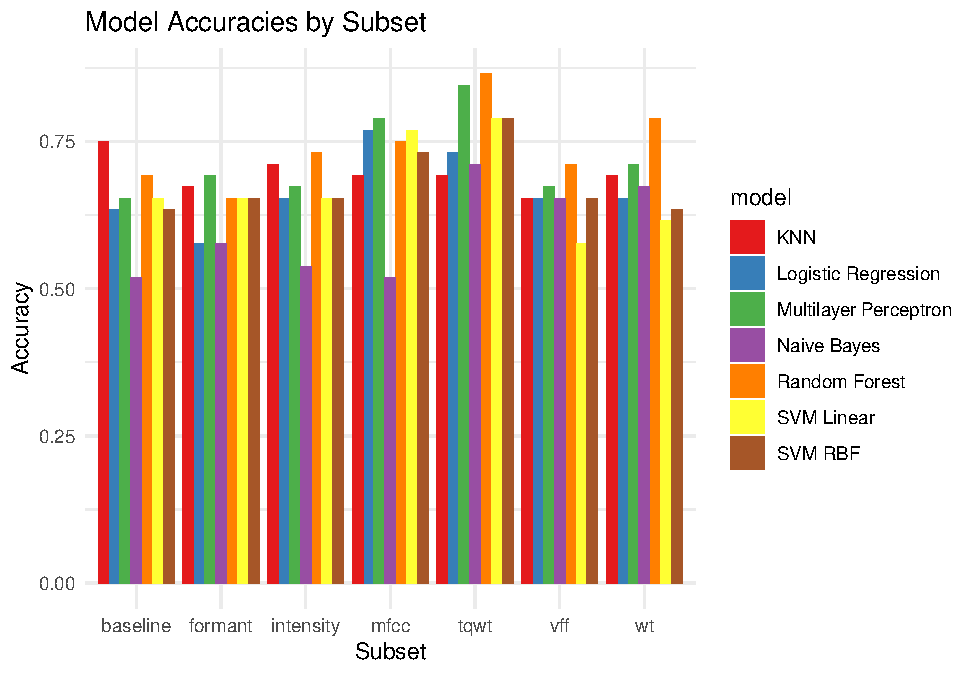
\includegraphics[width=1\linewidth,height=1\textheight]{figure/subfeatureresults-1} 

}

\caption{\label{fig:subfeatureresults}Sub-Feature Results by Algorithm }\label{fig:subfeatureresults}
\end{figure}

\newpage

\hypertarget{ensemble-accuracy-determination}{%
\subsection{Ensemble Accuracy Determination}\label{ensemble-accuracy-determination}}

At this point, we have enough data to make an ensemble predictive model, such that the best performing akgorithm for each sub-feature can be used. We used a similar method as the \textbf{Sakar et. al} paper, where a combination of weights and predictions are used to develop the ensemble model \(Y\):

\begin{equation}
Y = \sum w_i \cdot d_i
\label{eq:weighted_sum}
\end{equation}

\begin{equation}
w_i = \frac{\text{individual model weight}}{\text{sum of all model weights}}
\end{equation}

\begin{equation}
d_i = prediction_algorithm
\end{equation}

\begin{Shaded}
\begin{Highlighting}[]
\CommentTok{\# Functions for Ensemble predictions}
\NormalTok{weighted\_prediction }\OtherTok{\textless{}{-}} \ControlFlowTok{function}\NormalTok{(best\_models, test\_data, chosen\_features) \{}
\NormalTok{  predictions\_list }\OtherTok{\textless{}{-}} \FunctionTok{mapply}\NormalTok{(}\ControlFlowTok{function}\NormalTok{(subset\_name, model, test\_data, chosen\_features) \{}
    \ControlFlowTok{if}\NormalTok{ (}\FunctionTok{inherits}\NormalTok{(model, }\StringTok{"list"}\NormalTok{) }\SpecialCharTok{\&\&} \SpecialCharTok{!}\FunctionTok{is.null}\NormalTok{(model}\SpecialCharTok{$}\NormalTok{k)) \{ }\CommentTok{\# KNN model}
\NormalTok{      common\_columns }\OtherTok{\textless{}{-}} \FunctionTok{intersect}\NormalTok{(}\FunctionTok{colnames}\NormalTok{(test\_data[[subset\_name]]), }\FunctionTok{colnames}\NormalTok{(model}\SpecialCharTok{$}\NormalTok{train\_data))}
\NormalTok{  \} }\ControlFlowTok{else} \ControlFlowTok{if}\NormalTok{ (}\FunctionTok{class}\NormalTok{(model}\SpecialCharTok{$}\NormalTok{finalModel) }\SpecialCharTok{==} \StringTok{"ranger"}\NormalTok{) \{ }\CommentTok{\# Ranger model}
\NormalTok{      common\_columns }\OtherTok{\textless{}{-}} \FunctionTok{intersect}\NormalTok{(}\FunctionTok{colnames}\NormalTok{(test\_data[[subset\_name]]), model}\SpecialCharTok{$}\NormalTok{finalModel}\SpecialCharTok{$}\NormalTok{forest}\SpecialCharTok{$}\NormalTok{independent.variable.names)}
\NormalTok{  \} }\ControlFlowTok{else} \ControlFlowTok{if}\NormalTok{ (}\FunctionTok{inherits}\NormalTok{(model, }\StringTok{"nn"}\NormalTok{)) \{ }\CommentTok{\# Neural Network model}
\NormalTok{      common\_columns }\OtherTok{\textless{}{-}} \FunctionTok{intersect}\NormalTok{(}\FunctionTok{colnames}\NormalTok{(test\_data[[subset\_name]]), }\FunctionTok{colnames}\NormalTok{(model}\SpecialCharTok{$}\NormalTok{data))}
\NormalTok{  \} }\ControlFlowTok{else}\NormalTok{ \{}
    \FunctionTok{stop}\NormalTok{(}\StringTok{"Unsupported model type"}\NormalTok{)}
\NormalTok{  \}}
\NormalTok{    test\_subset\_data }\OtherTok{\textless{}{-}}\NormalTok{ test\_data[[subset\_name]][, common\_columns]}
    
    \ControlFlowTok{if}\NormalTok{ (}\FunctionTok{inherits}\NormalTok{(model, }\StringTok{"glm"}\NormalTok{)) \{}
      \FunctionTok{predict}\NormalTok{(model, }\AttributeTok{newdata =}\NormalTok{ test\_subset\_data, }\AttributeTok{type =} \StringTok{"response"}\NormalTok{)}
\NormalTok{    \} }\ControlFlowTok{else} \ControlFlowTok{if}\NormalTok{ (}\FunctionTok{class}\NormalTok{(model}\SpecialCharTok{$}\NormalTok{finalModel) }\SpecialCharTok{==} \StringTok{"ranger"}\NormalTok{) \{}
      \FunctionTok{predict}\NormalTok{(model, }\AttributeTok{newdata =}\NormalTok{ test\_subset\_data, }\AttributeTok{type =} \StringTok{"raw"}\NormalTok{)}
\NormalTok{    \} }\ControlFlowTok{else} \ControlFlowTok{if}\NormalTok{ (}\FunctionTok{inherits}\NormalTok{(model, }\StringTok{"svm"}\NormalTok{)) \{}
      \FunctionTok{predict}\NormalTok{(model, }\AttributeTok{newdata =}\NormalTok{ test\_subset\_data, }\AttributeTok{probability =} \ConstantTok{TRUE}\NormalTok{)}\SpecialCharTok{$}\NormalTok{probabilities[, }\DecValTok{2}\NormalTok{, drop }\OtherTok{=} \ConstantTok{FALSE}\NormalTok{]}
\NormalTok{    \} }\ControlFlowTok{else} \ControlFlowTok{if}\NormalTok{ (}\FunctionTok{inherits}\NormalTok{(model, }\StringTok{"naiveBayes"}\NormalTok{)) \{}
      \FunctionTok{predict}\NormalTok{(model, }\AttributeTok{newdata =}\NormalTok{ test\_subset\_data, }\AttributeTok{type =} \StringTok{"raw"}\NormalTok{)[, }\DecValTok{1}\NormalTok{, drop }\OtherTok{=} \ConstantTok{FALSE}\NormalTok{]}
\NormalTok{    \} }\ControlFlowTok{else} \ControlFlowTok{if}\NormalTok{ (}\FunctionTok{inherits}\NormalTok{(model, }\StringTok{"nn"}\NormalTok{)) \{}
\NormalTok{      predictions }\OtherTok{\textless{}{-}} \FunctionTok{compute}\NormalTok{(model, test\_subset\_data)}\SpecialCharTok{$}\NormalTok{net.result}
\NormalTok{      threshold\_func }\OtherTok{\textless{}{-}} \ControlFlowTok{function}\NormalTok{(x) }\FunctionTok{ifelse}\NormalTok{(x }\SpecialCharTok{\textgreater{}} \FloatTok{0.5}\NormalTok{, }\DecValTok{1}\NormalTok{, }\DecValTok{0}\NormalTok{)}
\NormalTok{      factor\_predictions }\OtherTok{\textless{}{-}} \FunctionTok{sapply}\NormalTok{(predictions, threshold\_func)}
      \FunctionTok{as.factor}\NormalTok{(factor\_predictions)}
\NormalTok{    \} }\ControlFlowTok{else} \ControlFlowTok{if}\NormalTok{ (}\FunctionTok{inherits}\NormalTok{(model, }\StringTok{"list"}\NormalTok{) }\SpecialCharTok{\&\&} \SpecialCharTok{!}\FunctionTok{is.null}\NormalTok{(model}\SpecialCharTok{$}\NormalTok{k)) \{}
      \FunctionTok{knn}\NormalTok{(}\AttributeTok{train =}\NormalTok{ model}\SpecialCharTok{$}\NormalTok{train\_data, }\AttributeTok{test =}\NormalTok{ test\_subset\_data, }\AttributeTok{cl =}\NormalTok{ model}\SpecialCharTok{$}\NormalTok{train\_class, }\AttributeTok{k =}\NormalTok{ model}\SpecialCharTok{$}\NormalTok{k)}
\NormalTok{    \} }\ControlFlowTok{else}\NormalTok{ \{}
      \FunctionTok{stop}\NormalTok{(}\StringTok{"Unsupported model type"}\NormalTok{)}
\NormalTok{    \}}
\NormalTok{  \}, }\AttributeTok{subset\_name =} \FunctionTok{names}\NormalTok{(best\_models), }\AttributeTok{model =} \FunctionTok{lapply}\NormalTok{(best\_models, }\StringTok{\textasciigrave{}}\AttributeTok{[[}\StringTok{\textasciigrave{}}\NormalTok{, }\StringTok{"model"}\NormalTok{), }\AttributeTok{test\_data =} \FunctionTok{rep}\NormalTok{(}\FunctionTok{list}\NormalTok{(test\_data), }\FunctionTok{length}\NormalTok{(}\FunctionTok{names}\NormalTok{(best\_models))), }\AttributeTok{chosen\_features =}\NormalTok{ chosen\_features, }\AttributeTok{SIMPLIFY =} \ConstantTok{FALSE}\NormalTok{)}
  
  \CommentTok{\# Convert factors to numeric values}
\NormalTok{  predictions\_list }\OtherTok{\textless{}{-}} \FunctionTok{lapply}\NormalTok{(predictions\_list, }\ControlFlowTok{function}\NormalTok{(x) }\FunctionTok{as.numeric}\NormalTok{(x)}\SpecialCharTok{{-}}\DecValTok{1}\NormalTok{)}

  \CommentTok{\# Calculate normalized weights}
\NormalTok{  models\_weights }\OtherTok{\textless{}{-}} \FunctionTok{lapply}\NormalTok{(best\_models, }\ControlFlowTok{function}\NormalTok{(x) x}\SpecialCharTok{$}\NormalTok{accuracy)}
\NormalTok{  models\_weights\_normalized }\OtherTok{\textless{}{-}} \FunctionTok{unlist}\NormalTok{(models\_weights) }\SpecialCharTok{/} \FunctionTok{sum}\NormalTok{(}\FunctionTok{unlist}\NormalTok{(models\_weights))}

  
  \CommentTok{\# Calculate weighted predictions}
\NormalTok{  combined\_probs }\OtherTok{\textless{}{-}} \FunctionTok{Reduce}\NormalTok{(}\StringTok{\textasciigrave{}}\AttributeTok{+}\StringTok{\textasciigrave{}}\NormalTok{, }\FunctionTok{mapply}\NormalTok{(}\StringTok{\textasciigrave{}}\AttributeTok{*}\StringTok{\textasciigrave{}}\NormalTok{, predictions\_list, models\_weights\_normalized, }\AttributeTok{SIMPLIFY =} \ConstantTok{FALSE}\NormalTok{))}
\NormalTok{  combined\_predictions }\OtherTok{\textless{}{-}} \FunctionTok{ifelse}\NormalTok{(combined\_probs }\SpecialCharTok{\textgreater{}} \FloatTok{0.5}\NormalTok{, }\DecValTok{1}\NormalTok{, }\DecValTok{0}\NormalTok{)}

  \FunctionTok{return}\NormalTok{(combined\_predictions)}
\NormalTok{\}}
\end{Highlighting}
\end{Shaded}

\newpage

Weights, as shown in Equation \ref{eq:weighted_sum}, are as follows:

\begin{table}

\caption{\label{tab:unnamed-chunk-9}Weighted Results and Selected Models per Sub-Feature}
\centering
\begin{tabular}[t]{llr}
\toprule
  & Subfeature & Weights\\
\midrule
Logistic Regression & baseline & 0.1347518\\
Random Forest & intensity & 0.1595745\\
SVM Linear & formant & 0.1453901\\
SVM RBF & vff & 0.1453901\\
Multilayer Perceptron & mfcc & 0.1560284\\
\addlinespace
Naive Bayes & wt & 0.1312057\\
KNN & tqwt & 0.1276596\\
\bottomrule
\end{tabular}
\end{table}

\newpage

\hypertarget{results}{%
\section{Results}\label{results}}

The results of the ensemble model on test data predictions are found below. These results are also compiled in the \textbf{test\_results.csv} file.\\

\begin{table}
\centering\begingroup\fontsize{10}{12}\selectfont

\begin{tabular}{cccccccc}
\toprule
ID...1 & Result...2 & ID...3 & Result...4 & ID...5 & Result...6 & ID...7 & Result...8\\
\midrule
63 & 1 & 61 & 1 & 67 & 1 & 73 & 1\\
44 & 1 & 10 & 1 & 68 & 0 & 25 & 1\\
29 & 1 & 37 & 1 & 30 & 1 & 48 & 1\\
9 & 1 & 57 & 1 & 15 & 1 & 74 & 1\\
38 & 1 & 8 & 1 & 18 & 1 & 50 & 1\\
\addlinespace
59 & 1 & 52 & 1 & 46 & 1 & 33 & 1\\
4 & 1 & 58 & 1 & 19 & 1 & 26 & 1\\
28 & 1 & 31 & 1 & 23 & 1 & 20 & 1\\
62 & 1 & 13 & 1 & 76 & 1 & 72 & 1\\
65 & 1 & 47 & 1 & 43 & 1 & 32 & 1\\
\addlinespace
69 & 1 & 36 & 1 & 22 & 1 & 3 & 0\\
39 & 1 & 56 & 1 & 53 & 1 & 51 & 1\\
1 & 1 & 54 & 1 & 27 & 1 & 60 & 1\\
11 & 1 & 70 & 1 & 75 & 1 & 35 & 1\\
40 & 1 & 16 & 1 & 21 & 1 & 34 & 1\\
\addlinespace
41 & 1 & 45 & 1 & 71 & 0 & 17 & 1\\
12 & 0 & 24 & 1 & 7 & 1 & 55 & 1\\
64 & 1 & 14 & 0 & 66 & 1 & 2 & 1\\
5 & 1 & 42 & 1 & 49 & 1 & 6 & 1\\
\bottomrule
\end{tabular}
\endgroup{}
\end{table}

\end{document}
